% ============================================================
%  State Debt Crisis: New York and Pennsylvania, 1813–1860
%  Composite document combining:
%   - state_defaults_1840s.tex  (analytical framing)
%   - new_york_1813_1860.tex    (New York detail)
%   - pennsylvania_1820_1860.tex (Pennsylvania detail)
% ============================================================
\documentclass[11pt]{article}

\usepackage{appendix}
\usepackage{amsmath,amssymb,amsthm,enumerate,epsfig}
\usepackage{ifthen,latexsym}
\usepackage{fullpages}
\usepackage{comment}
\usepackage{booktabs}
\usepackage{tabularx}
\usepackage{subcaption}
\usepackage[Figure sright]{rotating}
\usepackage{color,colortbl}
\definecolor{LightCyan}{rgb}{0.88,1,1}
\usepackage[round,comma,authoryear]{natbib}
\usepackage{caption,subcaption}
\usepackage{setspace}
\usepackage[margin=1in]{geometry}
\usepackage{hyperref}

\bibliographystyle{mynat}
\bibpunct{(}{)}{,}{a}{}{,}

\onehalfspacing

% ------ macros ------
\newcommand{\Lower}[1]{\smash{\lower 1.5ex \hbox{#1}}}
\newcommand{\STRUT}{\rule{0in}{3ex}}
\newcommand{\BSTRUT}{\rule[-1.2ex]{0pt}{0pt}}
\newcommand{\TS}[1]{{\textcolor{red}{#1}}}
\newcommand{\GH}[1]{{\textcolor{blue}{#1}}}

% ------ theorems ------
\newtheorem{theorem}{Theorem}[section]
\newtheorem{remark}[theorem]{Remark}
\newtheorem{proposition}[theorem]{Proposition}
\newtheorem{lemma}[theorem]{Lemma}
\newtheorem{definition}[theorem]{Definition}

%%%%%%%%%%%%%%%%%%%%%%%%%%%%%%%%%%%%%%%%%%%%%%%%%%%%%%%%%%%

\title{Taxless Finance and Its Consequences:\\
New York and Pennsylvania, 1813--1860\footnote{We thank William Berkley
for supporting our research.  Hall thanks the Theodore and Jane Norman Fund for
financial support.}}

\author{George J.\ Hall\footnote{Brandeis University,
  \texttt{ghall@brandeis.edu}.} \and
Thomas J.\ Sargent\footnote{New York University,
  \texttt{thomas.sargent@nyu.edu}.}}

\date{\today}

%%%%%%%%%%%%%%%%%%%%%%%%%%%%%%%%%%%%%%%%%%%%%%%%%%%%%%%%%%%

\begin{document}
\graphicspath{{figures/}{Penn_figures/}}

\maketitle

\begin{abstract}
\noindent
In the early 1840s multiple U.S.\ states defaulted on bonds issued to
finance infrastructure projects, precipitating a wave of constitutional
reforms that fundamentally reshaped state fiscal institutions.  This
paper examines New York and Pennsylvania as the ``good'' and ``bad''
case studies in that episode.  Drawing on annual fiscal records for
New York (1813--1860) and Pennsylvania (1820--1860), we trace how both
states pursued ``taxless finance''---borrowing against anticipated toll
revenues without raising current taxes---and how their differing fiscal
structures led to sharply different outcomes: New York narrowly avoided
default while Pennsylvania defaulted in 1842.  We then document the
constitutional responses adopted by both states that eliminated the
taxless-finance option and established fiscal constraints still
influential in American public finance today.
\end{abstract}

\newpage
\tableofcontents
\newpage

%============================================================
\section{Introduction}
\label{sec:intro}
%============================================================

In the early 1840s, the United States experienced a sovereign debt crisis at
the state level.  Nine states and one territory defaulted on bond obligations
following the Panic of 1837, marking one of the most significant fiscal crises
in American history.  This crisis led to fundamental constitutional reforms in
multiple states, with New York and Pennsylvania among those adopting strict
limitations on state borrowing and prohibitions on the pledging of state credit
to private enterprises.

The defaults were concentrated among states that had borrowed heavily to finance
``internal improvements''---primarily canals and railroads---using what economic
historians term \emph{taxless finance}.  Rather than raising property taxes to
fund infrastructure, states borrowed against anticipated toll revenues and hoped
that increased land values would eventually generate sufficient tax receipts to
service the debt \citep{wallis2005constitutions}.  When the economic depression
following the Panic of 1837 reduced both toll revenues and land values, states
that had relied on this strategy found themselves unable to service their debts.

New York and Pennsylvania make ideal paired case studies.  Both states invested
heavily in canal systems in the 1820s and 1830s; both accumulated large debts;
both faced severe fiscal pressure in the early 1840s.  Yet their outcomes
differed sharply.  New York---whose Erie Canal was an extraordinary commercial
success---narrowly avoided default, while Pennsylvania defaulted in 1842 and
remained in default until 1845.  The contrast illuminates both the role of
project quality and the role of pre-existing fiscal institutions.

The remainder of this paper is organized as follows.  Section~\ref{sec:framework}
presents the government budget constraints that organize our fiscal analysis.
Sections~\ref{sec:newyork} and~\ref{sec:pennsylvania} provide detailed fiscal
portraits of New York and Pennsylvania, respectively.  Section~\ref{sec:compare}
places the two states in comparative perspective.  Section~\ref{sec:constitution}
documents the constitutional responses.  Section~\ref{sec:taxless} analyzes the
taxless-finance problem.  Section~\ref{sec:longrun} discusses long-run impact,
and Section~\ref{sec:conclusion} concludes.

%============================================================
\section{Analytical Framework: Government Budget Constraints}
\label{sec:framework}
%============================================================

The organizing principle for our fiscal analysis is the government budget
constraint with private assets (``state funds''):
\begin{eqnarray}
\underbrace{G_t}_{\substack{\text{government}\\\text{spending}}}
  + \underbrace{r_t^B B_{t-1}}_{\substack{\text{interest on}\\\text{state debt}}}
  + \underbrace{A_t - A_{t-1}}_{\substack{\text{change in}\\ \text{state funds}}}
  &=& \underbrace{T_t}_{\text{taxes}}
     + \underbrace{r_t^A A_{t-1}}_{\substack{\text{interest on}\\ \text{state funds}}}
     + \underbrace{B_t - B_{t-1}}_{\substack{\text{change in}\\ \text{state debt}}}
\label{eq:consolidated_bc}
\end{eqnarray}
This consolidated constraint holds for both states,
though their accounting structures differ: New York maintained
separate ``Canal'' and ``General'' accounts, while Pennsylvania
recorded public-works spending and revenues within a single general account.

\subsection{New York: Three Budget Constraints}

New York's separate Canal Commission accounting requires us to decompose the
consolidated constraint~\eqref{eq:consolidated_bc}.  The \emph{Canal Account}
satisfies:
\begin{eqnarray}
\underbrace{F^c_t - F^c_{t-1}}_{\substack{\text{change in}\\ \text{Canal Fund}}}
  &=& \underbrace{B^c_t - B^c_{t-1}}_{\text{new Canal Debt}}
    + \underbrace{TOLL^c_t}_{\text{tolls}}
    + \underbrace{T^c_t}_{\text{taxes}}
    + \underbrace{OR^c_t}_{\text{other revenue}}
    + \underbrace{TR^{gc}_t}_{\substack{\text{transfers from}\\ \text{General Account}}}
    \nonumber \\
  &&
    + \, \underbrace{r_t^A F^c_{t-1}}_{\substack{\text{interest on}\\ \text{Canal Fund}}}
    - \underbrace{EXP^c_t}_{\text{Canal expenses}}
    - \underbrace{r_t^B B^c_{t-1}}_{\substack{\text{interest on}\\ \text{Canal debt}}}
    - \underbrace{TR^{cg}_t}_{\substack{\text{transfers to}\\ \text{General Account}}}
\label{eq:canal_bc}
\end{eqnarray}

The \emph{General Account} satisfies:
\begin{eqnarray}
\underbrace{F^g_t - F^g_{t-1}}_{\substack{\text{change in}\\ \text{General Fund}}}
  &=& \underbrace{B^g_t - B^g_{t-1}}_{\substack{\text{change in}\\ \text{General Debt}}}
    + \underbrace{T^g_t}_{\text{taxes}}
    - \underbrace{TR^{gc}_t}_{\substack{\text{transfer to}\\ \text{Canal Account}}}
    + \underbrace{r_t^A F^g_{t-1}}_{\substack{\text{interest on}\\ \text{General Fund}}}
    \nonumber \\
  &&
    - \underbrace{S^g_t}_{\substack{\text{General Account}\\ \text{spending}}}
    - \underbrace{r_t^B B^g_{t-1}}_{\substack{\text{interest on}\\ \text{General Fund debt}}}
    + \underbrace{TR^{cg}_t}_{\substack{\text{transfers from}\\ \text{Canal Account}}}
\label{eq:general_bc}
\end{eqnarray}

Adding~\eqref{eq:canal_bc} and~\eqref{eq:general_bc} and defining
$A_t = F^c_t + F^g_t$,\; $B_t = B^c_t + B^g_t$,\;
$T_t = TOLL^c_t + T^c_t + T^g_t + OR^c_t$,\;
$G_t = S^g_t + EXP^c_t$
recovers the consolidated constraint~\eqref{eq:consolidated_bc}.

\subsection{Pennsylvania: One Budget Constraint}

Unlike New York, Pennsylvania included public-works spending and revenues
directly in its general account, so the consolidated constraint applies directly
with $A_t$ capturing the Commonwealth's holdings of bank stocks, turnpike
stocks, and canal and navigation stocks.

%============================================================
\section{New York State, 1813--1860: The ``Good'' Case}
\label{sec:newyork}
%============================================================

\subsection{Overview}

New York presents the more favorable outcome in the state debt crisis.
Several features distinguish it from states that defaulted:

\begin{itemize}
\item In the 1790s and early 1800s, New York legislators aspired to finance
  state government from permanent funds derived from land sales and special
  duties---a government ``without taxation.''  Later, with the opening of the
  Erie Canal, the state became largely a venture-capital operation.

\item New York paid off its pre-1814 debt by the mid-1820s but resumed
  borrowing to pay for ordinary expenditures in the 1830s.

\item New York borrowed heavily to finance the construction and maintenance
  of the Canal System, with canals representing the dominant share of
  state debt throughout this period.

\item In the late 1830s and early 1840s, New York faced two major fiscal
  shocks: (i) three railroad companies whose debt was guaranteed by the State
  went bankrupt, and (ii) a state-run bank insurance system collapsed when 11
  banks failed.

\item Despite these shocks, New York did not default on its debt during the
  crisis of the 1840s.  Its bonds traded at a discount, and the Comptroller
  complained publicly---but coupon and principal payments were maintained.

\item New York adopted a new constitution in 1846 that fundamentally changed
  the rules governing state borrowing.

\item There are important connections to Hamilton's 1790 federal assumption of
  state war debts, which formed the foundation of New York's General Fund.
  There are also recurring unit-of-account issues during periods of paper
  currency.
\end{itemize}

\subsection{State Funds}
\label{sec:ny_funds}

\subsubsection{Origins: Hamilton's 1790 Settlement}

In the 1780s, New York held substantial Revolutionary War debts.  It also
held the following Continental Securities:

\begin{center}
\begin{tabular}{lr}
State Holdings of Continental Securities & Amount~(£~s~d) \\
\hline
Loan Office Certificates             & 360,683 9 3\STRUT\\
Certificates, Wm.~Barber            & 458,213 4 0\\
Certificates, Pierce, Burrel, Deming & 389,498 9 9\\
Indent of Interest                   & 2,502 14 8 \\
\hline
Total & 1,210,897 16 8\STRUT
\end{tabular}
\end{center}

In 1791, Alexander Hamilton exchanged these securities for:
\begin{center}
\begin{tabular}{lr}
United States 6\% Stock          & \$898,847.03 \\
United States deferred 6\% stock & \$520,688.66 \\
United States 3\% Stock          & \$680,681.70 \\
\hline
Total                            & \$2,100,197.39
\end{tabular}
\end{center}
(Source: \citet[pp.~255--6]{Sowers_1914}.)  The accounts between the State and
the Secretary of the Treasury were finally settled in 1800.

These three stocks formed the basis of what became known as the \textit{General
Fund}.  The Comptroller was made custodian and was empowered to invest it;
over time, the fund was augmented from sales of public lands and other sources.

\subsubsection{The Six Major Funds}

Between 1813 and 1860, New York maintained six major funds and eight minor
sinking funds:

\begin{enumerate}
\item The \textit{General Fund} was created from the 1790 federal settlement
  and augmented with asset sales; it helped fund ordinary government but its
  principal was gradually drawn down and ultimately replaced by debt.

\item The \textit{Canal Fund} was financed by the revenues of the Erie Canal
  and other canals and used to pay canal expenses and Canal Fund debts.

\item The \textit{Common School Fund} was a permanent endowment fund for
  public education, established in 1805 from the proceeds of the first 500,000
  acres of vacant land managed by the Surveyor-General.  No direct state tax
  for school purposes was levied until 1853; from 1805 to 1853, the interest
  on the fund---supplemented by the U.S.\ Deposit Fund---supported the state's
  system of free public education.  The fund grew from \$0.82 million in 1813
  to \$2.6 million in 1860.

\item The \textit{Literature Fund} (est.\ 1827) supported secondary education
  and the creation of libraries in\emph{ academies}.  Unlike the Common School
  Fund, which supported free local schools, the Literature Fund served
  privately governed academies charging tuition.  It was eventually
  consolidated with the U.S.\ Deposit Fund.

\item The \textit{Bank Safety Fund} (described below) was a bank insurance
  fund that went insolvent after 11 banks failed between 1840 and 1842.

\item The \textit{U.S.\ Deposit Fund} was created after the federal government
  distributed its fiscal surplus to the states under the Deposit Act of 1836.
  The money was lent by the state secured by real-estate mortgages; interest
  supported the Common School Fund.
\end{enumerate}

The eight minor sinking funds were created following the state's assumption of
debts from three failed railroads (see Section~\ref{sec:ny_debt}).

In Figure~\ref{fig:fund_balances}, we plot the balances for these funds.

\begin{figure}[htbp]
\center{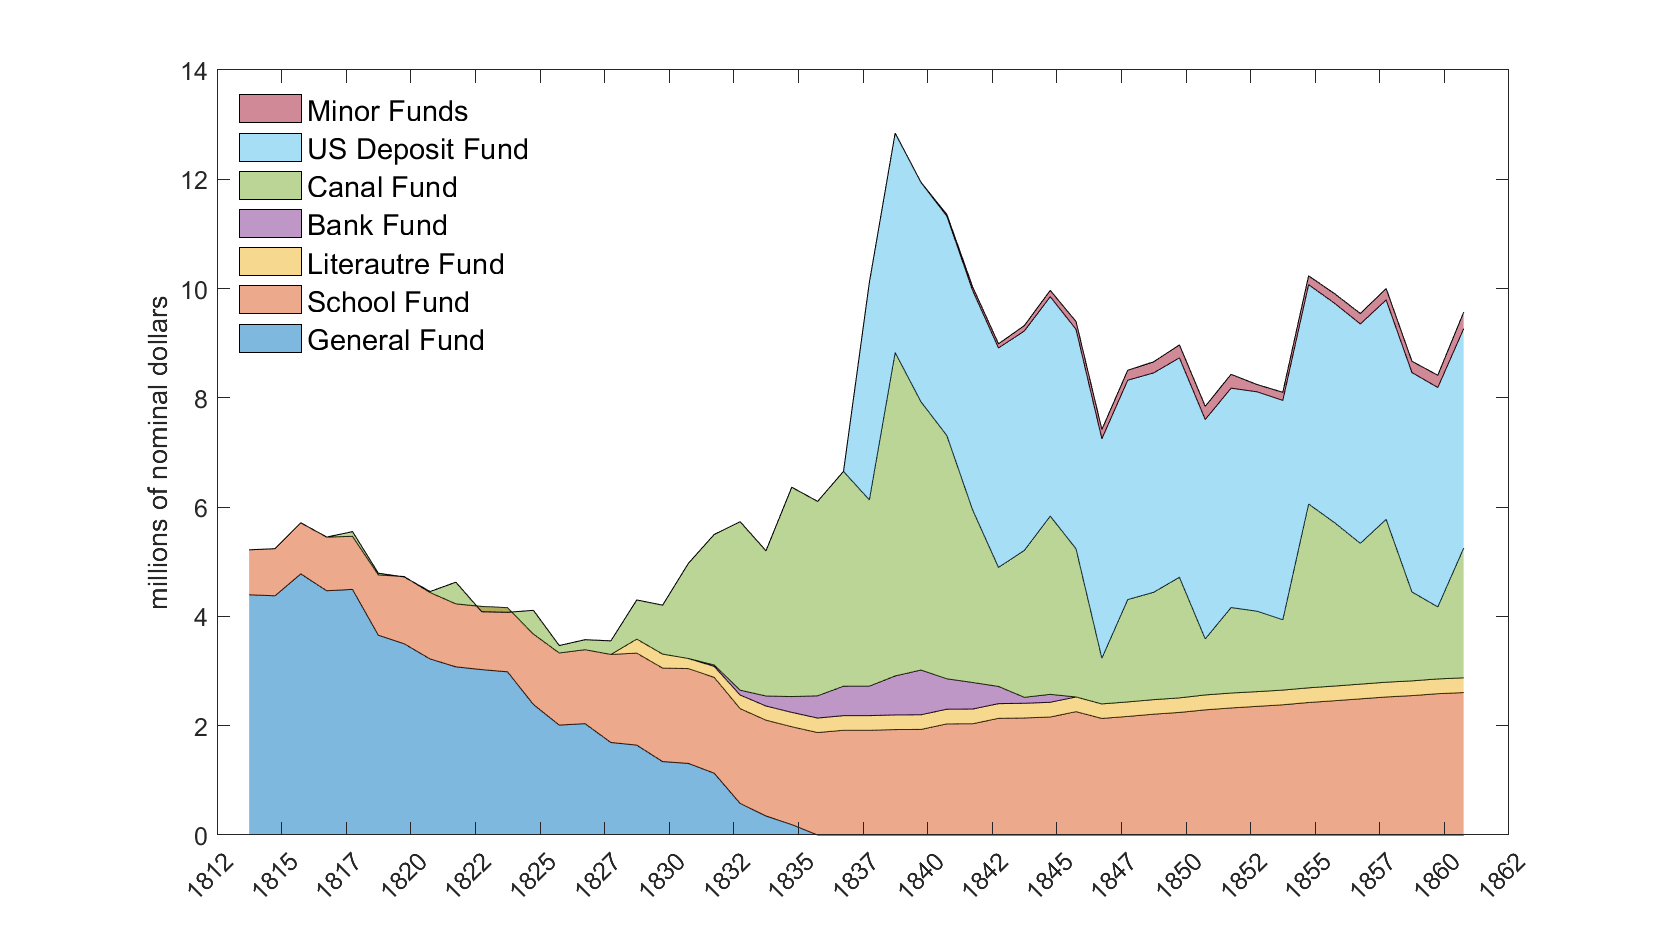
\includegraphics[scale=0.50]{fund_balances.png}}
\caption{New York State Fund Balances}
\label{fig:fund_balances}
\end{figure}

\subsubsection{The Bank Safety Fund}

In 1829, New York established a bank insurance system, the \emph{Bank Safety
Fund}.  Banks were required to deposit securities in the Comptroller's office
as guaranty for their circulating notes, with annual assessments of
$\frac{1}{2}$ of 1\% of paid-in capital until each bank had contributed 3\%.
The fund would reimburse creditors of any failing bank.

Albert Gallatin observed presciently:
\begin{quote}
\ldots with the laudable intent to protect the community against partial
failures, a `safety fund' has been established by law \ldots which is
applicable to the payments of the notes of any that may fail.  This must have
the tendency to encourage excessive issues of paper, which could not be
sustained if resting only on the credit of the bank by which they are made.
\citep{Bodenhorn_1996}
\end{quote}

Between February~1840 and October~1842, eleven banks failed (Table~\ref{table:failed_banks}).
The total cost of insuring their creditors was \$2.565 million; the fund became
insolvent in 1843.

\begin{table}[htbp]
\centering\small
\begin{tabular}{lrrrrr}
                               &          &           & Other     & Receipts    & Balance \\
                               & Date of  & Notes     & Debts     & from Asset  & Paid by \\
Failed Bank                    & Failure  & Redeemed  & Paid      & Sales       & Fund \\
\hline
City Bank of Buffalo           & 2/1840   & \$317,107 &           & \$99,996    & \$217,111\STRUT \\
Wayne County Bank              & 12/1840  &   113,131 & \$16,078  &             &    129,209 \\
Commercial Bank of New York City& 9/1841  &   139,837 &   146,129 & \$7,188     &    278,778 \\
Bank of Buffalo                & 11/1841  &   435,540 &   149,241 &             &    584,781 \\
Commercial Bank of Buffalo     & 11/1841  &   186,861 &   424,515 &   5,000     &    606,376 \\
Commercial Bank of Oswego      & 12/1841  &   163,162 &    78,352 &   2,392     &    239,122 \\
Watervliet Bank                & 3/1842   &   134,107 &    77,484 &  13,258     &    198,333 \\
Clinton County Bank            & 4/1842   &    71,896 &   156,257 &             &    228,153 \\
Bank of Lyons                  & 9/1842   &    52,898 &    40,053 &   3,761     &     88,990 \\
Lafayette Bank, NYC            & 2/1842   &        38 &           &             &         38 \\
Oswego Bank                    & 10/1842  &       725 &           &   6,482     &          - \\
\hline
Total                          &          & \$1,615,302 & \$1,088,109 & \$138,077 & \$2,565,334\STRUT \\
\end{tabular}
\caption{Payments Made by the Bank Safety Fund to Reimburse Creditors of the Failed Banks}
\label{table:failed_banks}
\flushleft{\footnotesize Source: \citet[p.~332]{Chaddock_1910} and
  \citet[p.~25]{Bodenhorn_1996}.}
\end{table}

\subsection{New York State Debts}
\label{sec:ny_debt}

Figure~\ref{fig:debt_balances} plots the quantity of New York State debt
outstanding.  There are three types: General Fund debt, Contingent debt, and
Canal debt.  Canal debt constitutes the lion's share.  About 42\% of the
total was held abroad.  Table~\ref{table:ny_state_debt_1841_42} reproduces the
ownership distribution from the 1842 Annual Report of the Comptroller.

\begin{figure}[htbp]
\center{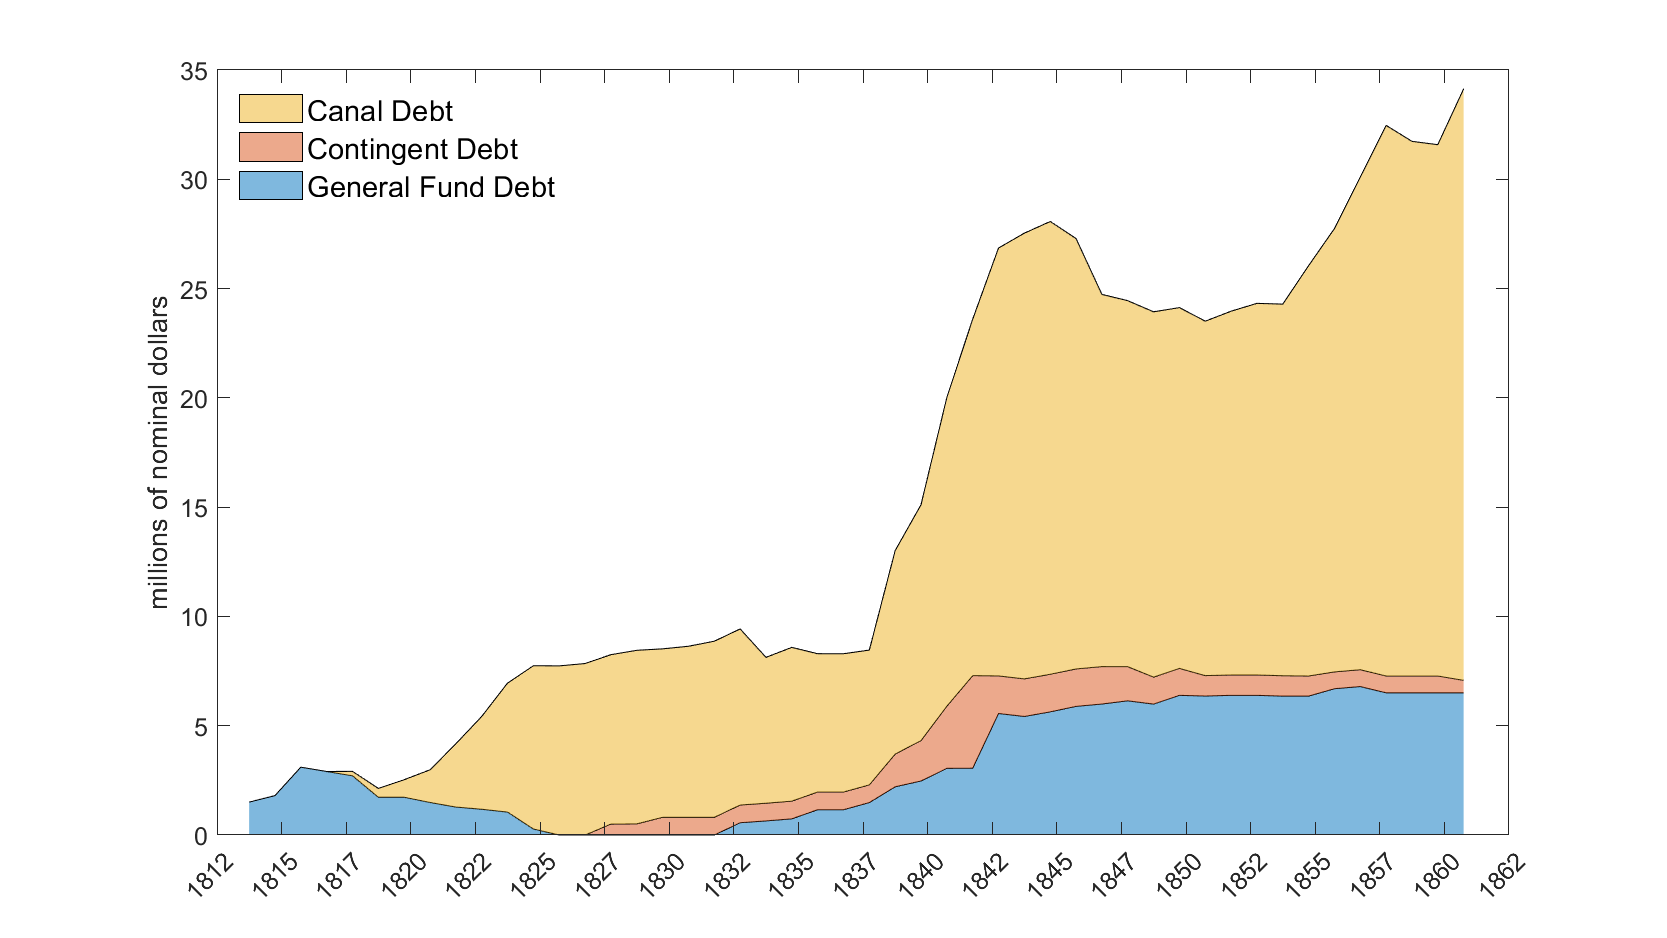
\includegraphics[scale=0.50]{debt_balances.png}}
\caption{New York State Debt}
\label{fig:debt_balances}
\end{figure}

\begin{table}[htbp]
\centering\small
\begin{tabular}{lrrrr}
      & \multicolumn{3}{c}{Held} \\
      \cline{2-4}
Bond  & in New York & in Other States & by Foreigners & Total\STRUT \\
\hline
Erie and Champlain Canals         & \$150,530  & \$18,495   & \$1,715,412  & \$1,884,437\STRUT\\
Enlargement of Erie Canal         & 3,294,049  & 333,229    & 3,407,341    & 7,034,619 \\
Cayuga, Seneca, and Oswego Canals & 376,079    & 26,211     & 256,014      & 658,304 \\
Crooked Lake Canal                & 114,000    & ---        & 5,500        & 120,000 \\
Chemung Canal                     & 156,007    & 5,700      & 314,707      & 476,974 \\
Chenango Canal                    & 629,232    & 223,392    & 1,549,911    & 2,402,536 \\
Black River Canal                 & 357,552    & 8,167      & 739,955      & 1,105,673 \\
Genesee Valley Canal              & 606,064    & 81,905     & 1,878,411    & 2,566,380 \\
Oneida River Improvement          & 43,800     & 1,200      & 5,000        & 50,000 \\
Oneida Lake Canal                 & 50,000     & ---        & ---          & 50,000 \\
7\% stock of 1848                 & 1,445,736  & 106,500    & 32,500       & 1,584,736 \\
7\% stock of 1849                 & 1,608,000  & 13,600     & 31,000       & 1,652,600 \\
Delaware \& Hudson Canal Co.      & 409,317    & 17,359     & 373,324      & 800,000 \\
New York \& Erie Railroad Co.     & 2,587,000  & 251,000    & 162,000      & 3,000,000 \\
Tonawanda Railroad                & 86,000     & 14,000     & ---          & 100,000 \\
Schenectady Railroad              & 100,000    & ---        & ---          & 100,000 \\
Long Island Railroad              & 80,000     & 3,000      & 17,000       & 100,000 \\
Catskill and Canajoharie Railroad & 86,000     & ---        & 114,000      & 200,000 \\
Ithaca and Owego Railroad         & 82,000     & 12,000     & 221,700      & 315,700 \\
Auburn and Rochester Railroad     & 188,000    & 11,000     & 1,000        & 200,000 \\
Hudson and Berkshire Railroad     & 141,000    & ---        & 9,000        & 150,000 \\
Tioga Coal, Iron and Mining Co.   & 70,000     & ---        & ---          & 70,000 \\
Astor Stock                       & 561,500    & ---        & ---          & 561,500 \\
5\% Bank Fund Stock               & 350,257    & ---        & ---          & 350,257 \\
7\% stock and bonds               & 465,358    & ---        & ---          & 465,358 \\
\hline
Total                         & \$14,038,540 & \$1,240,962 & \$10,833,776 & \$25,999,074\STRUT
\end{tabular}
\caption{Ownership Distribution of New York State Debts, 1841--42}
\label{table:ny_state_debt_1841_42}
\flushleft{\footnotesize Source: 1842 \emph{Annual Report of the Comptroller},
pp.~9--10.}
\end{table}

\subsubsection{General Fund Debt and the Assumption of Railroad Obligations}

General Fund debt appeared in 1814 alongside a positive General Fund balance;
it was paid off by 1825.  In 1832 the State resumed borrowing to cover ordinary
expenditures.

Starting in 1827, the State issued \emph{contingent debt}: bonds issued on
behalf of canal and railroad companies for which the State pledged its faith and
credit.  On July~1, 1841, the Ithaca and Owego and Catskill and Canajoharie
railroads ceased coupon payments; the New York and Erie Railroad subsequently
defaulted as well.  As a result, \$3,315,700 in railroad debt became a direct
State obligation.

\subsection{The Canal Account}

New York's Erie Canal, completed in 1825, was the dominant source of state
revenue and the primary driver of state debt.  Figures~\ref{fig:canal_revenue}--\ref{fig:canal_rev_out}
plot the Canal Account's revenues, expenditures, and their comparison.

\begin{itemize}

\item From 1817 to 1820, taxes on auctions, salt, and steamboat revenue
  constituted the sole Canal Account revenue.  Between 1817 and 1836 these
  taxes were diverted from the General Account to the Canal Account.

\item Although the Erie Canal officially opened on October~26, 1825, toll
  collection began in 1821.  By the late 1820s tolls became the Canal's
  largest revenue source; revenues declined in the late 1830s and 1850s.

\item Prior to 1840, the Canal Account received transfers from the General Account.
  After 1840, the flow reversed: the Canal Account transferred surpluses back
  to the General Account (Figure~\ref{fig:canal_transfers}).

\end{itemize}

\begin{figure}[htbp]
\center{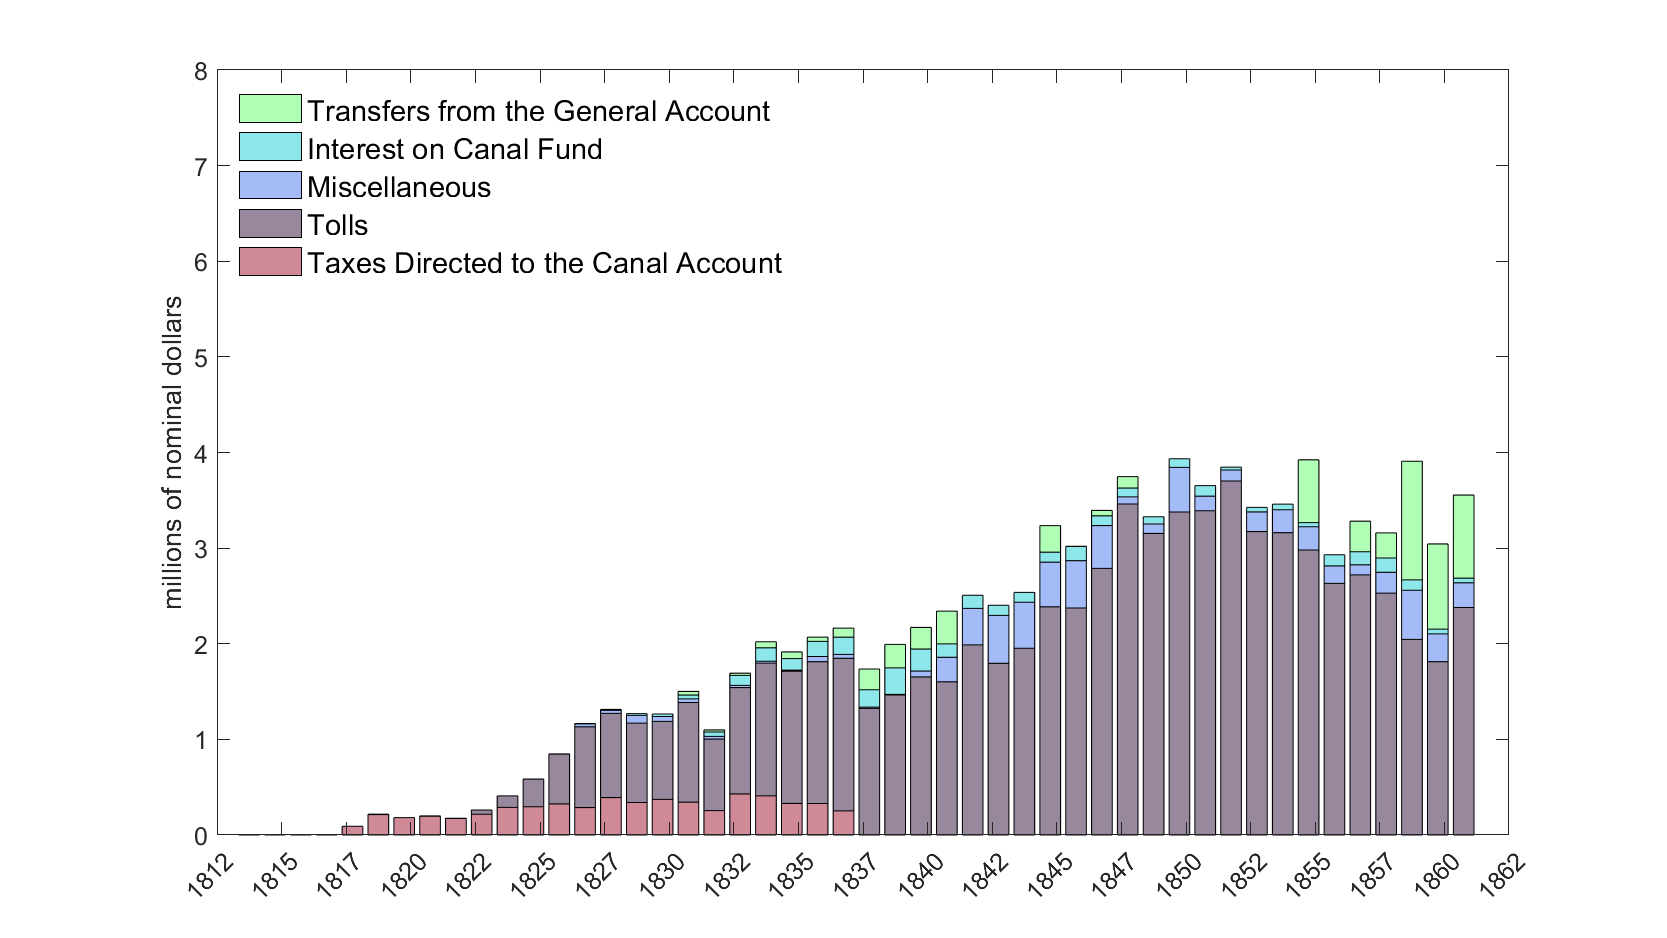
\includegraphics[scale=0.50]{canal_account_revenue.png}}
\caption{New York Canal Account Revenues}
\label{fig:canal_revenue}
\end{figure}

\begin{figure}[htbp]
\center{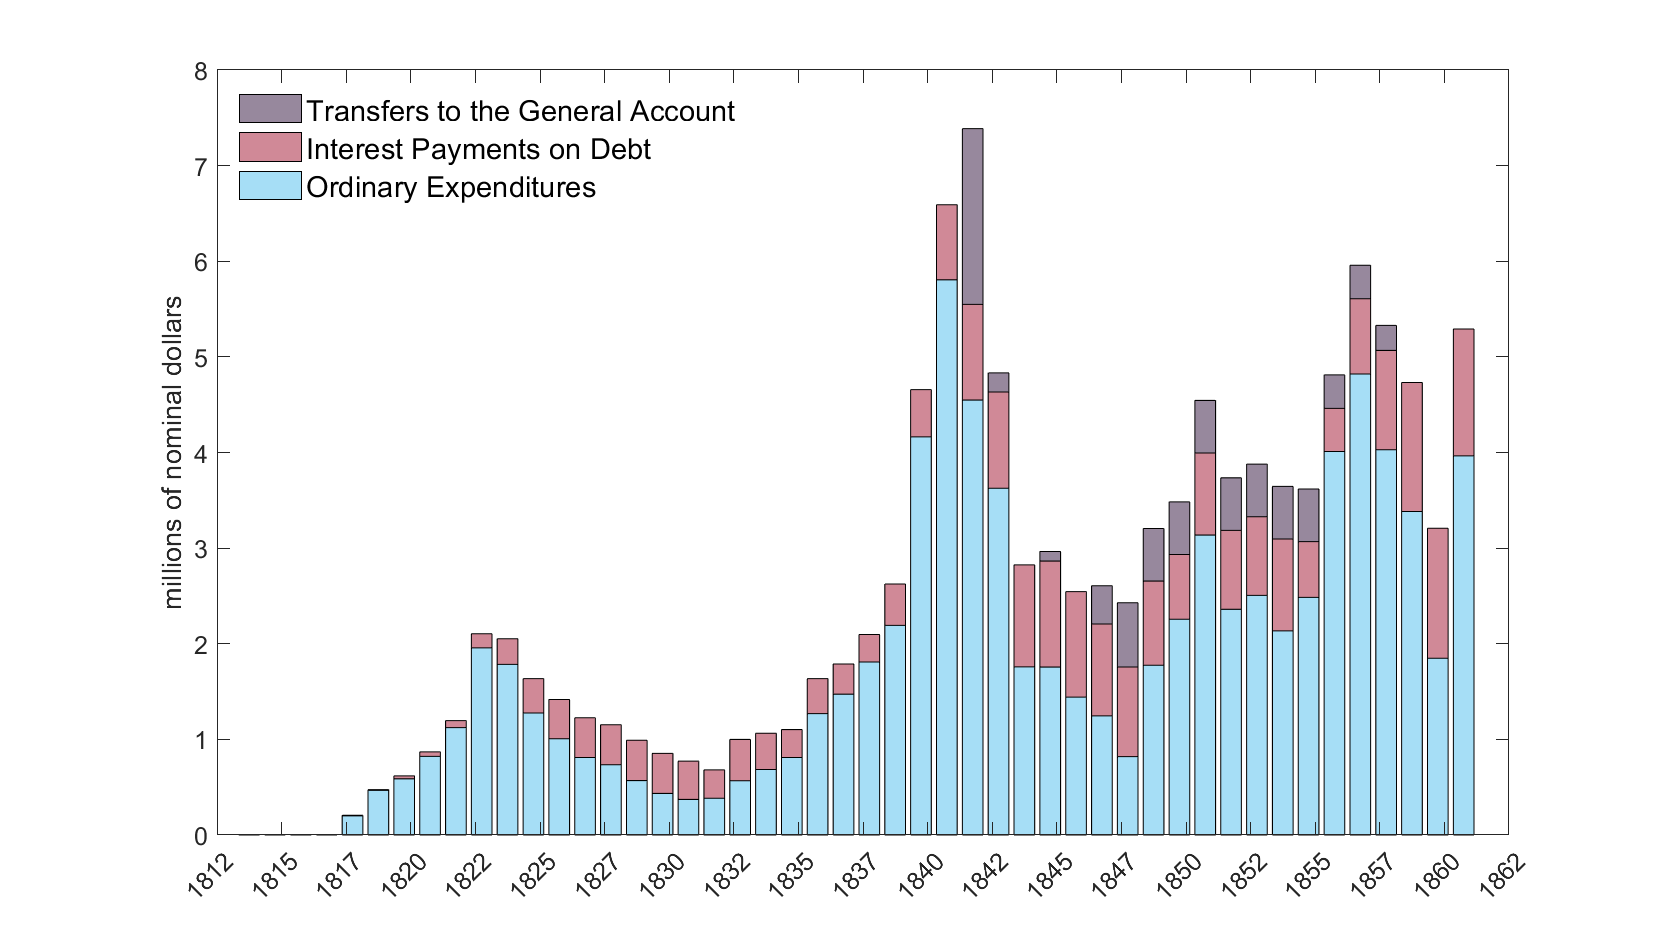
\includegraphics[scale=0.50]{canal_acct_spending.png}}
\caption{New York Canal Account Expenditures}
\label{fig:canal_outlays}
\end{figure}

\begin{figure}[htbp]
\center{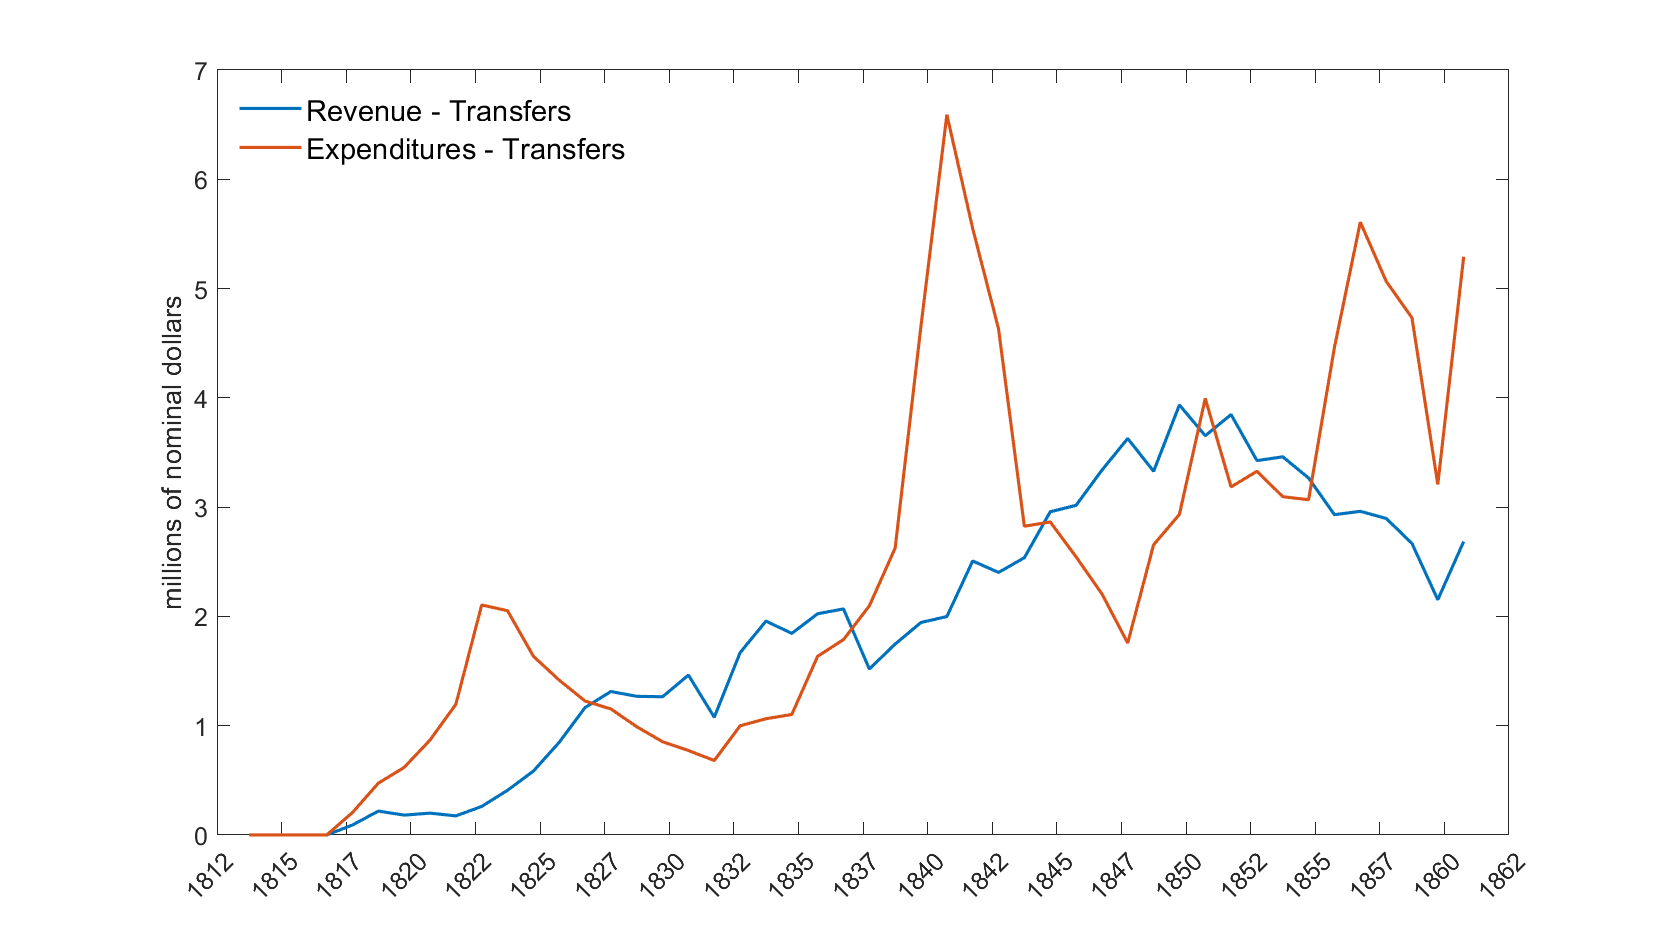
\includegraphics[scale=0.50]{erie_canal_revenue_outlays.png}}
\caption{New York Canal Account Revenue and Expenditures (net of inter-account transfers)}
\label{fig:canal_rev_out}
\end{figure}

\begin{figure}[htbp]
\center{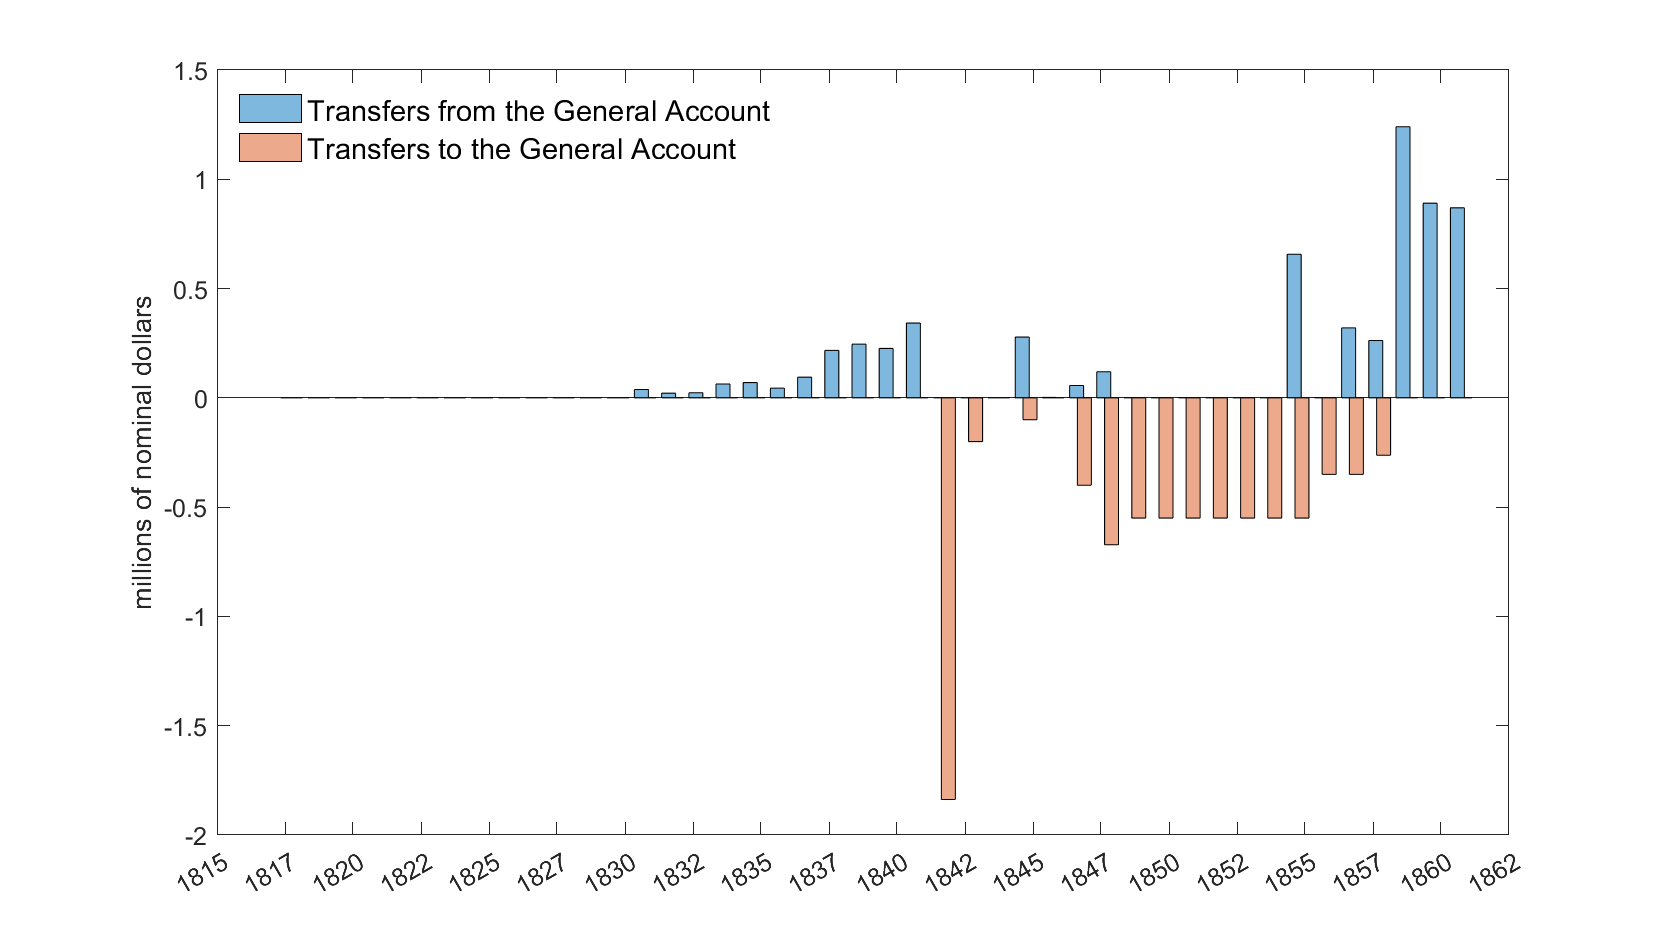
\includegraphics[scale=0.50]{erie_canal_transfers_tofrom_general_fund.png}}
\caption{Transfers Between the Canal and General Accounts}
\label{fig:canal_transfers}
\end{figure}

\subsection{The General Account}

\begin{itemize}

\item A state property tax was in effect between 1816 and 1826, accounting for
  a large share of General Account revenue.  It was reinstated in 1842 in
  response to the fiscal crisis.

\item During the late 1820s and early 1830s, revenue from the state accounts
  (primarily returns on the General Fund investment portfolio) made up the
  lion's share of General Account revenue.  In 1832 the State resumed
  borrowing for ordinary expenditures, signaling that investment income was
  no longer sufficient.

\item The 1836 distribution of the federal surplus under the Deposit Act
  provided a one-time revenue boost.

\item The assumption of contingent railroad debt in 1841--42 and the Bank
  Safety Fund payments to failed-bank creditors both raised General Account
  outlays sharply.

\end{itemize}

Figures~\ref{fig:general_acct_revenue}--\ref{fig:general_acct_rev_out} plot
General Account revenues, expenditures, and their comparison.

\begin{figure}[htbp]
\center{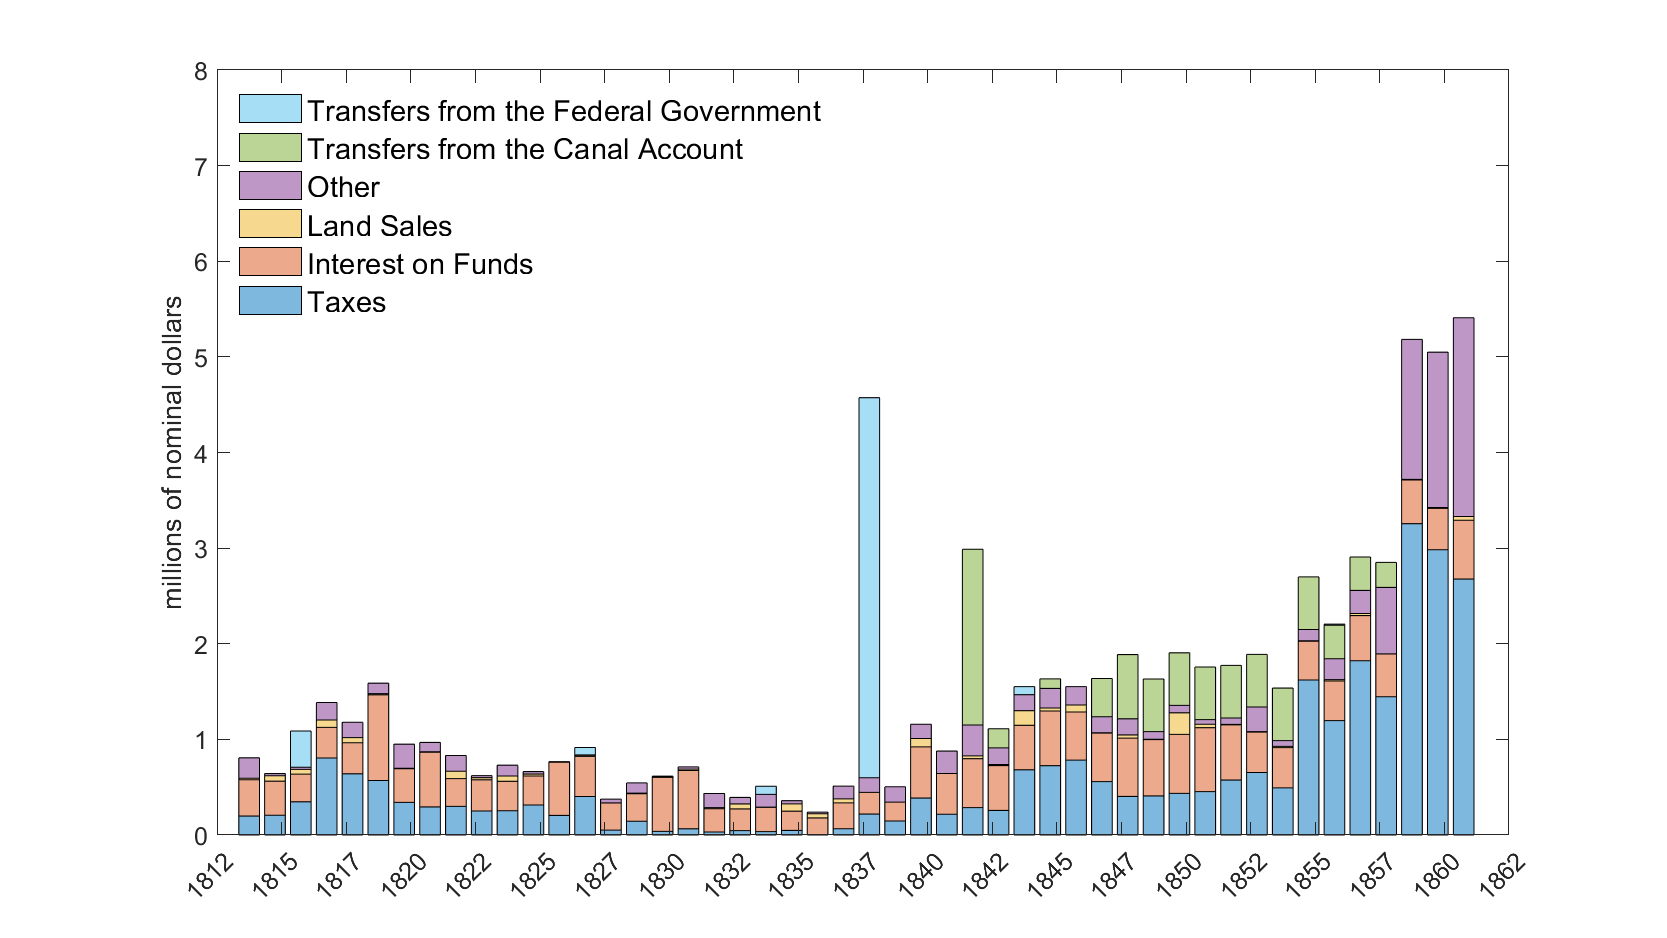
\includegraphics[scale=0.50]{general_account_revenue.png}}
\caption{General Account Revenues}
\label{fig:general_acct_revenue}
\end{figure}

\begin{figure}[htbp]
\center{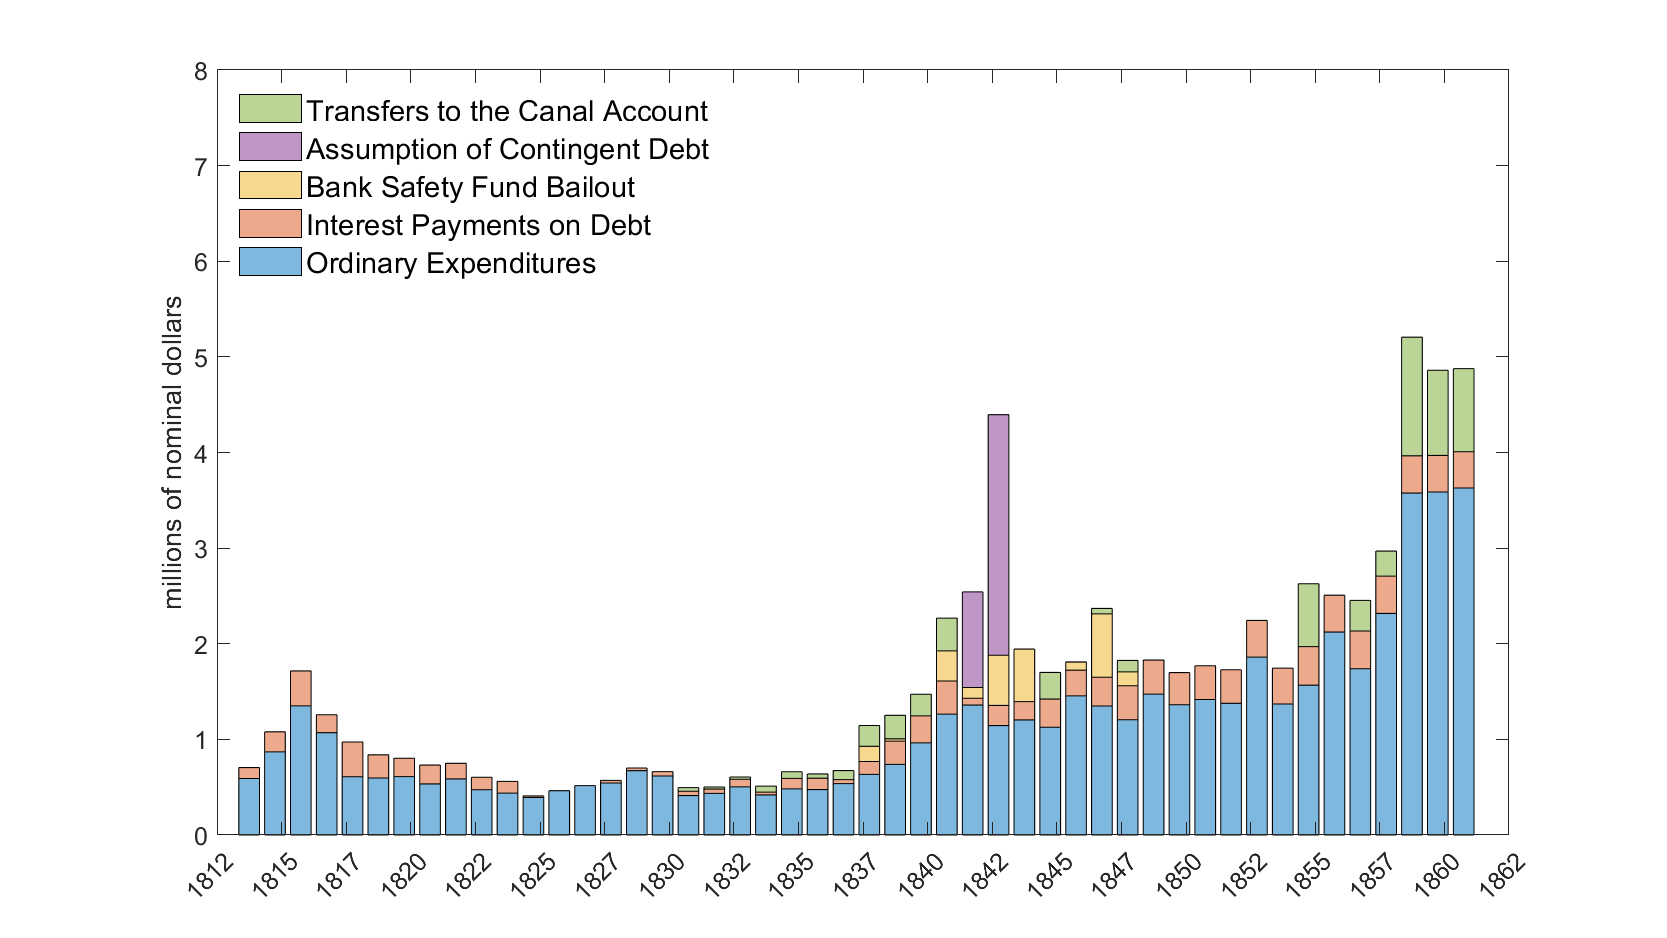
\includegraphics[scale=0.50]{general_acct_spending.png}}
\caption{General Account Expenditures}
\label{fig:general_acct_outlays}
\end{figure}

\begin{figure}[htbp]
\center{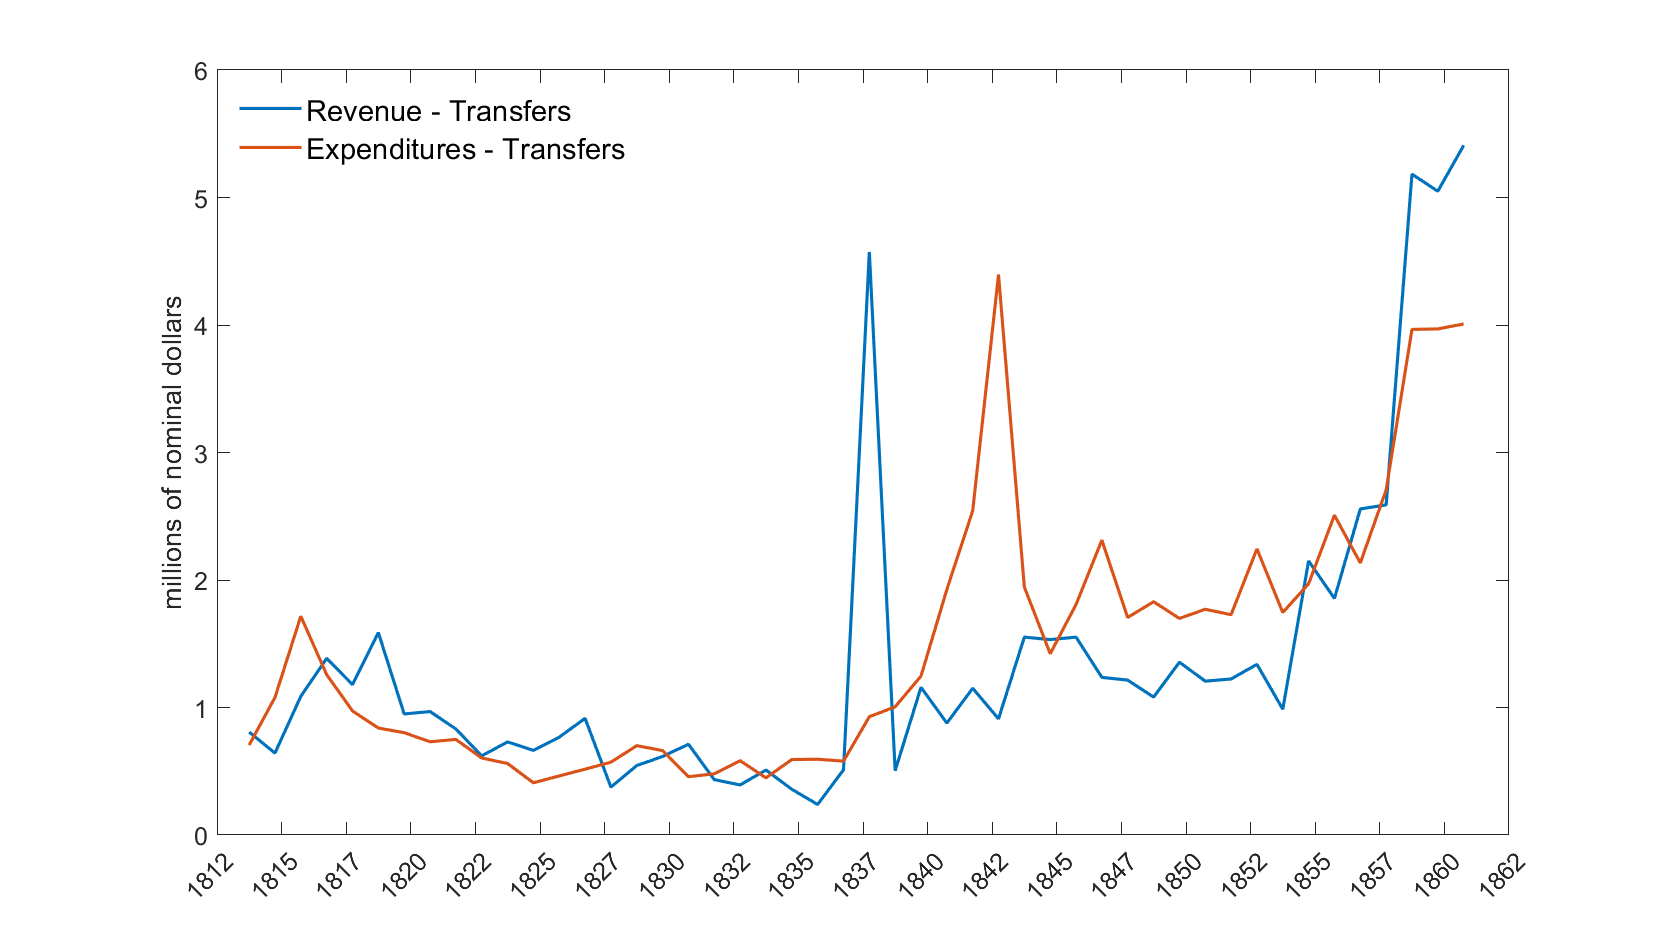
\includegraphics[scale=0.50]{general_acct_revenue_outlays.png}}
\caption{General Account Revenue and Expenditures}
\label{fig:general_acct_rev_out}
\end{figure}

\subsection{Consolidated Accounts}

Figures~\ref{fig:consolidated_revenue}--\ref{fig:consolidated_rev_out} merge
the Canal and General Accounts.  The Canal Account's revenues and expenditures
dwarf those of the General Account: New York State was primarily a canal
operator with a secondary role in ordinary government.  With the important
exception of the late 1830s and early 1840s, the consolidated budget was
broadly balanced.

\begin{figure}[htbp]
\center{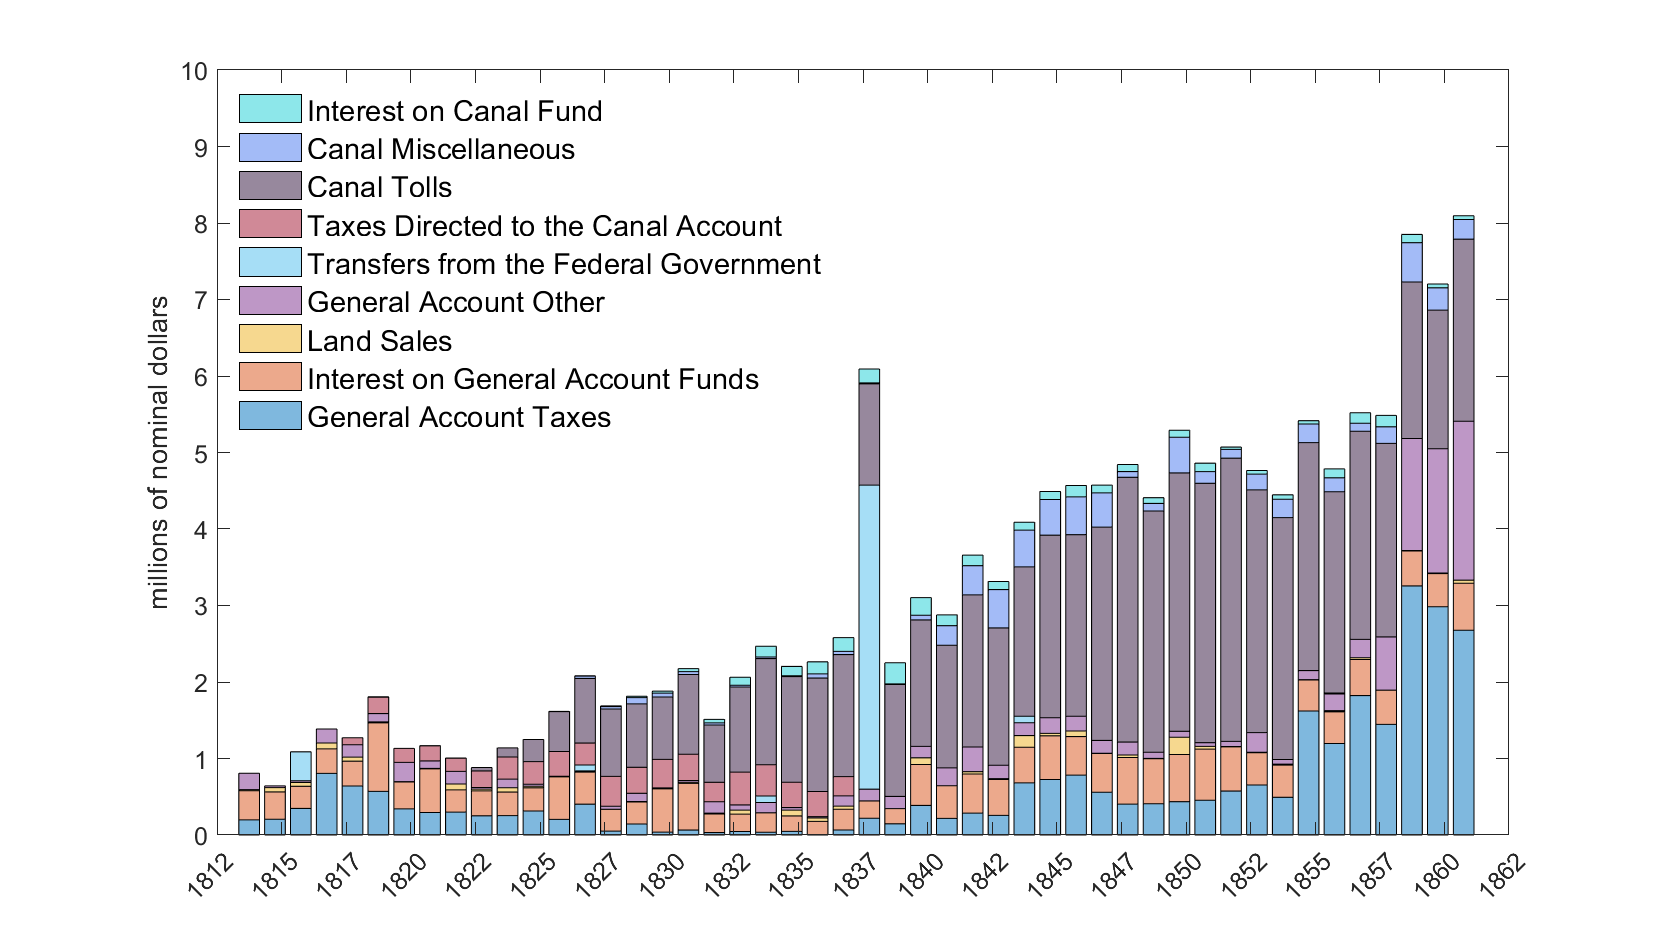
\includegraphics[scale=0.50]{consolidated_account_revenue.png}}
\caption{New York Consolidated Revenues}
\label{fig:consolidated_revenue}
\end{figure}

\begin{figure}[htbp]
\center{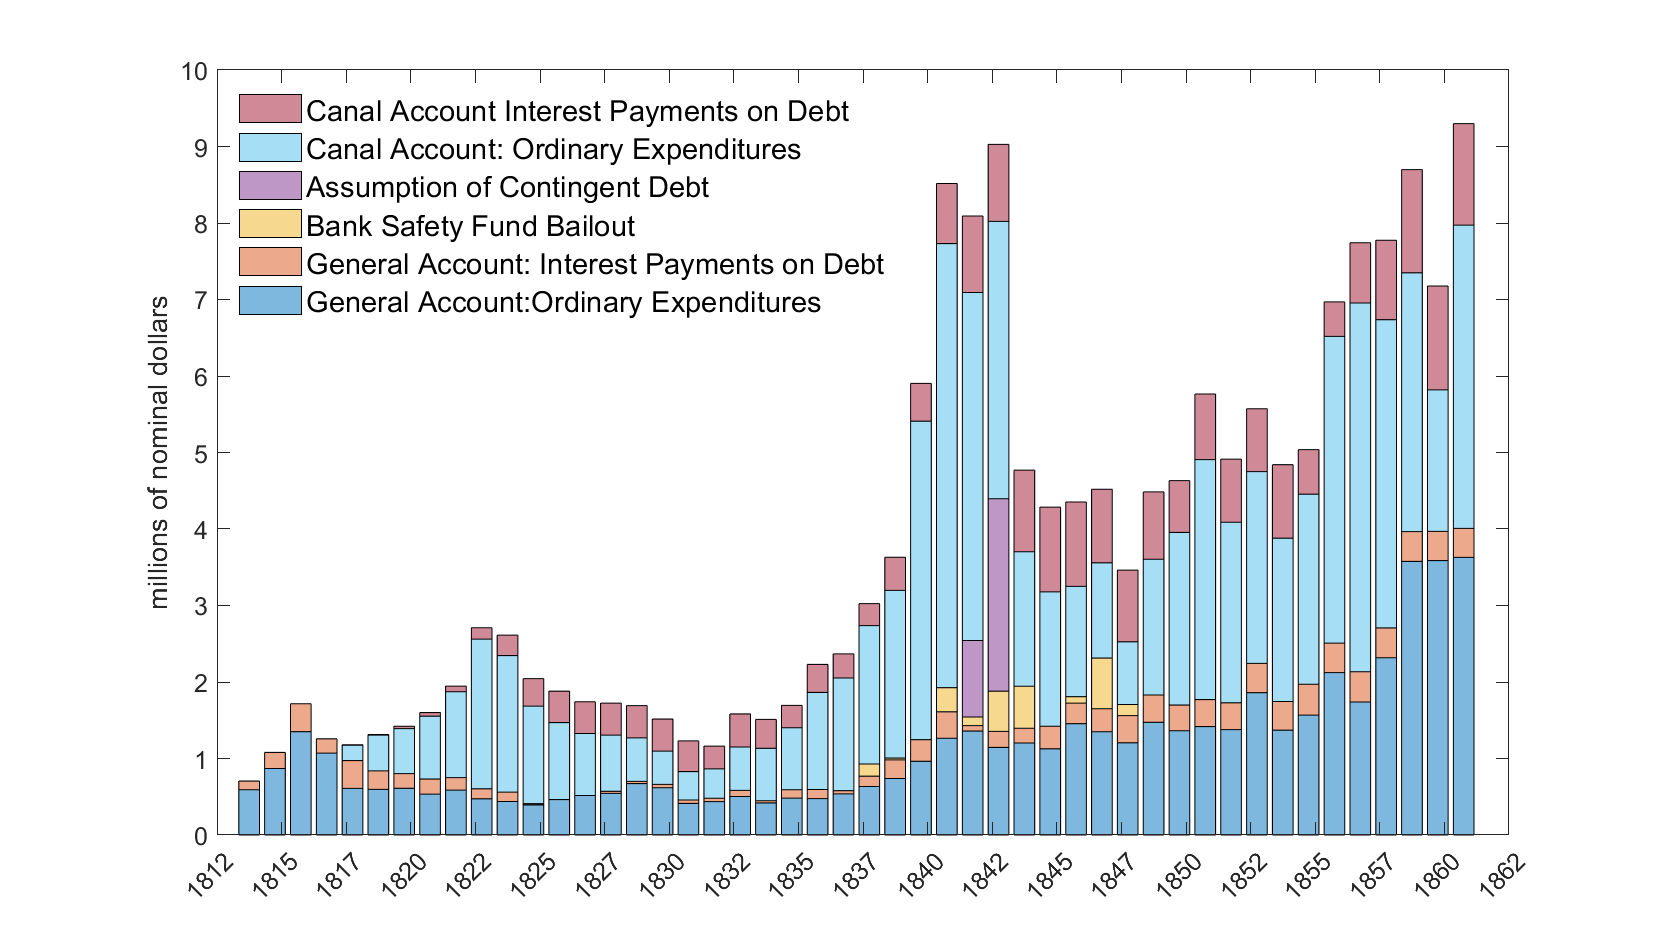
\includegraphics[scale=0.50]{consolidated_acct_spending.png}}
\caption{New York Consolidated Expenditures}
\label{fig:consolidated_outlays}
\end{figure}

\begin{figure}[htbp]
\center{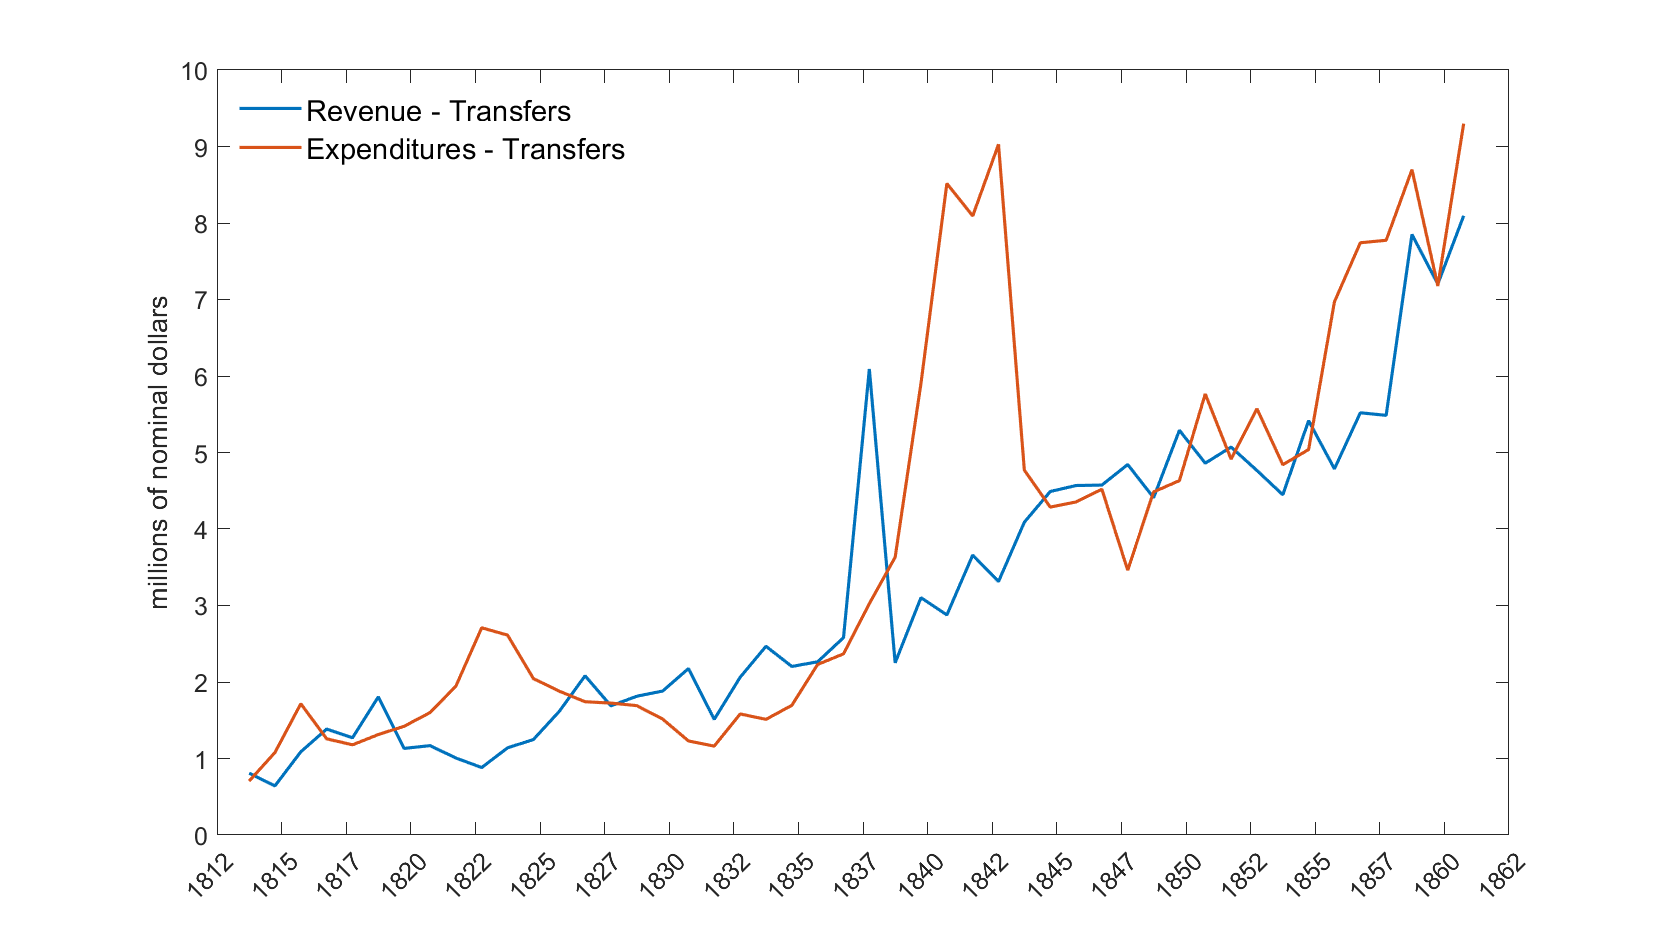
\includegraphics[scale=0.50]{consolidated_revenue_outlays.png}}
\caption{New York Consolidated Revenue and Expenditures}
\label{fig:consolidated_rev_out}
\end{figure}

\subsection{Bond Prices and Fiscal Stress}

Figure~\ref{fig:nys_bond_prices} plots the prices of three Canal bonds and
three General Fund bonds.

Despite never missing a coupon or principal payment, New York State bonds
traded at 80 cents on the dollar in the early 1840s.  Comptrollers complained
publicly about the discount.  The late 1830s and early 1840s were a period of
acute fiscal stress: the Legislature suspended all public works except those
whose suspension would cause a significant loss, and it pledged the state's
revenues for the payment of its obligations.

\begin{figure}[htbp]
\center{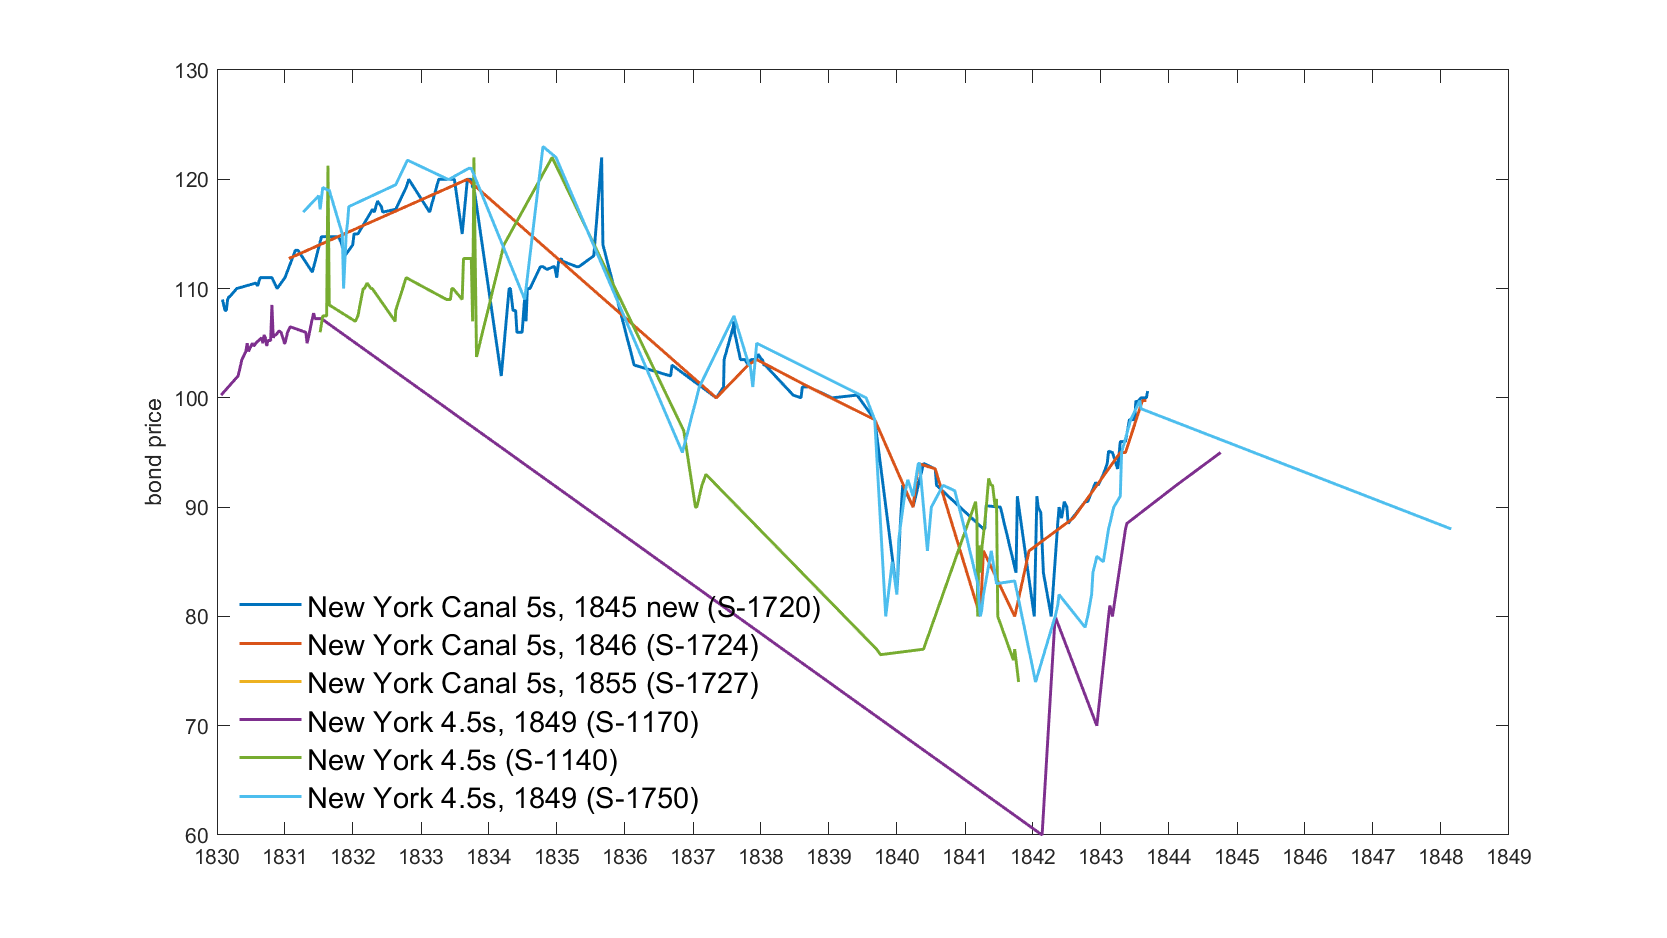
\includegraphics[scale=0.50]{ny_state_debt_prices.png}}
\caption{Prices of Various New York State Bonds}
\flushleft{\footnotesize Source: \cite{Sylla_Wilson_Wright}.}
\label{fig:nys_bond_prices}
\end{figure}

\subsection{Unit of Account Issues}

New York's fiscal record repeatedly intersected with monetary standard
questions:

\begin{itemize}
\item When specie payments were suspended during the financial panic of 1837,
  Comptroller Azariah C.\ Flagg used State resources to make up the difference
  between depreciated paper currency and coin, thus honoring the State's
  obligations at par.

\item In 1857, Comptroller William F.\ Allen urged that the State's bonded debt
  be serviced in coin rather than paper, arguing that the public faith of New
  York should not fluctuate with the market value of its currency.

\item During the Civil War, when specie commanded a substantial premium over
  paper, Comptroller Lucius Robinson recommended (in 1863 and 1864) that both
  principal and interest on the State's bonds be paid in specie.  The
  Legislature declined.

\item In 1870, the State entered the open market to purchase coin for interest
  payments, a practice continued until the federal government's general
  resumption of specie payments in 1879.  By adhering voluntarily to a
  metallic standard during the years of national paper currency, New York
  strengthened its credit-market standing and set a precedent for conservative
  financial management that endured well into the late nineteenth century.
\end{itemize}

%============================================================
\section{Pennsylvania, 1820--1860: The ``Bad'' Case}
\label{sec:pennsylvania}
%============================================================

\subsection{Overview}

Pennsylvania presents the unfavorable outcome.  Inspired by the early success
of New York's Erie Canal, Pennsylvania embarked on a more ambitious and
ultimately less successful program of state-sponsored internal improvements.
The Commonwealth borrowed heavily, maintained an aversion to direct taxation,
and defaulted in August~1842.  The contrast with New York captures in
miniature the broader cross-state patterns identified by \citet{wallis2005constitutions}.

Unlike New York, Pennsylvania included public-works spending and revenues
directly in its general account, a feature that both simplified the
accounting and obscured the true fiscal position.

\subsection{Revenues and Expenditures}

Figures~\ref{fig:penn_rev_exp}--\ref{fig:penn_expenditures} plot Pennsylvania's
revenues and expenditures.

\begin{itemize}

\item Spending on internal improvements and interest payments constituted by far
  the largest expenditure categories.

\item In 1842, 1843, and 1844, Pennsylvania failed to make promised interest
  and other payments.  Bondholders were issued ``interest certificates,'' while
  unpaid claims from government contractors were recorded as debts to
  ``domestic creditors.''

\item The 1836--37 spike in revenue reflects the federal distribution of surplus
  funds under the Deposit Act of 1836, together with unusually large fees from
  bank-charter enrollments.

\item After the crisis, the Commonwealth ran a primary surplus and achieved a
  broadly balanced gross budget.  Tax revenue increased substantially starting
  in 1845 as a large number of new taxes were introduced.

\item In 1840, Pennsylvania's debt stood at \$33.3 million and the State
  collected \$1.9 million in total revenue.  That same year, New York's
  consolidated debt was \$17.6 million and it collected \$2.9 million in total
  revenue---a substantially better debt-to-revenue ratio.

\end{itemize}

\begin{figure}[htbp]
\center{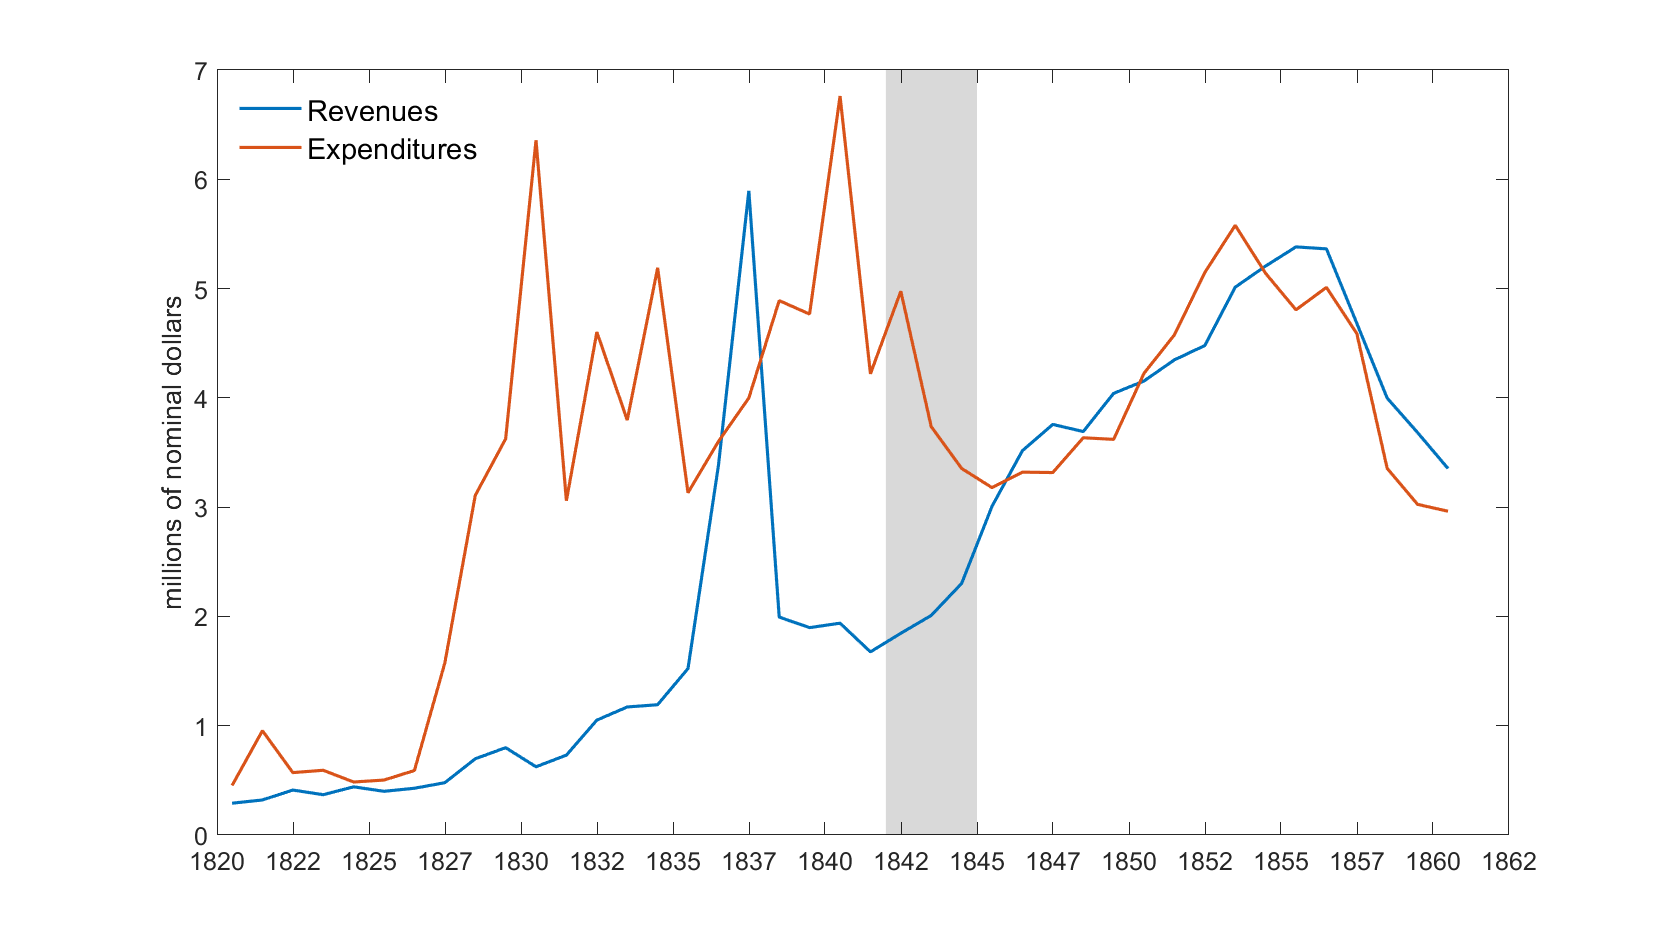
\includegraphics[scale=0.50]{penn_revenue_expend.png}}
\caption{Pennsylvania State Revenue and Expenditures}
\flushleft{\footnotesize The period of default (1842--1844) is shaded in grey.}
\label{fig:penn_rev_exp}
\end{figure}

\begin{figure}[htbp]
\center{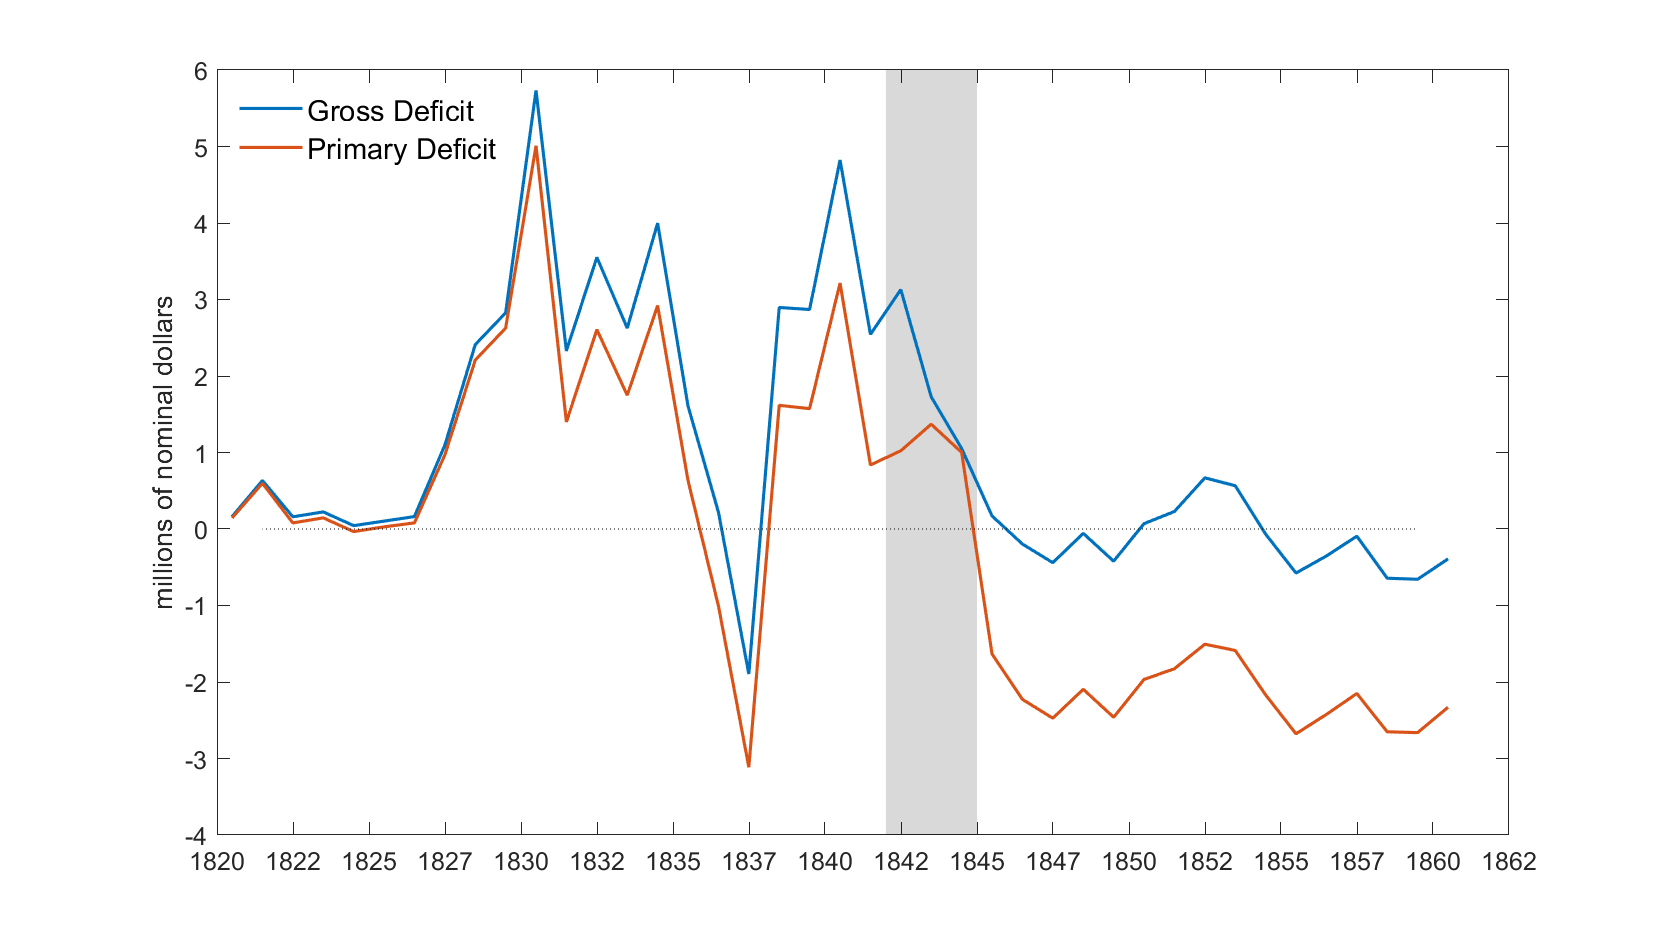
\includegraphics[scale=0.50]{penn_deficit.png}}
\caption{Pennsylvania Gross and Primary Deficits}
\flushleft{\footnotesize The period of default (1842--1844) is shaded in grey.}
\label{fig:penn_deficits}
\end{figure}

\begin{figure}[htbp]
\center{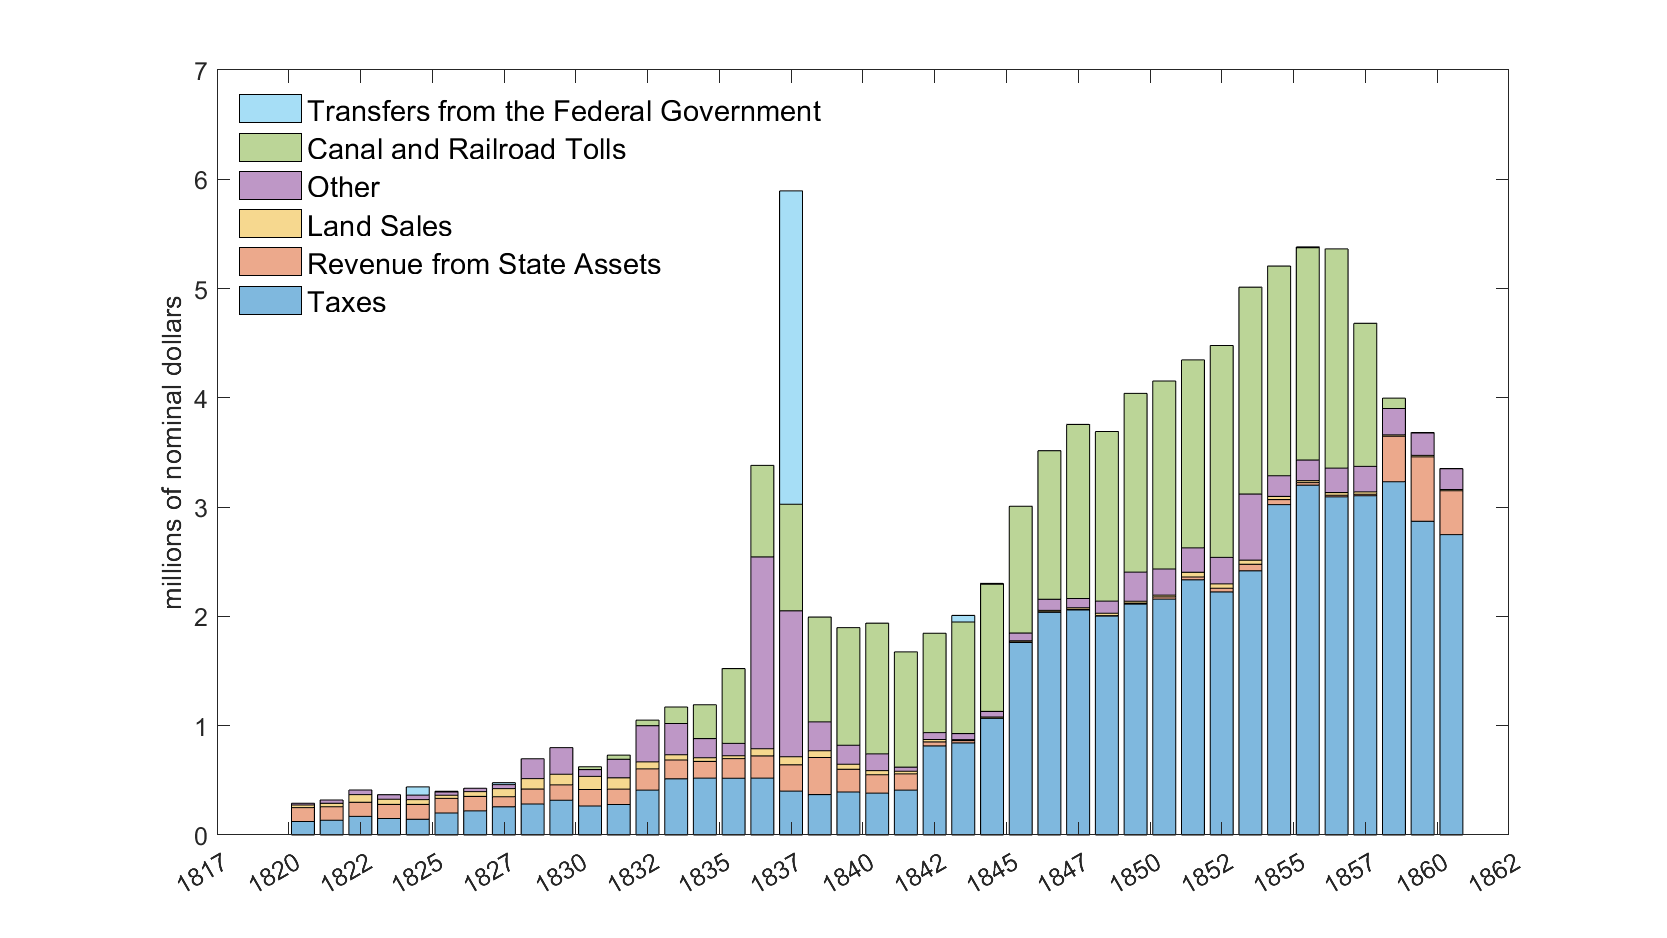
\includegraphics[scale=0.50]{penn_revenues.png}}
\caption{Pennsylvania Revenue Decomposed}
\label{fig:penn_revenues}
\end{figure}

\begin{figure}[htbp]
\center{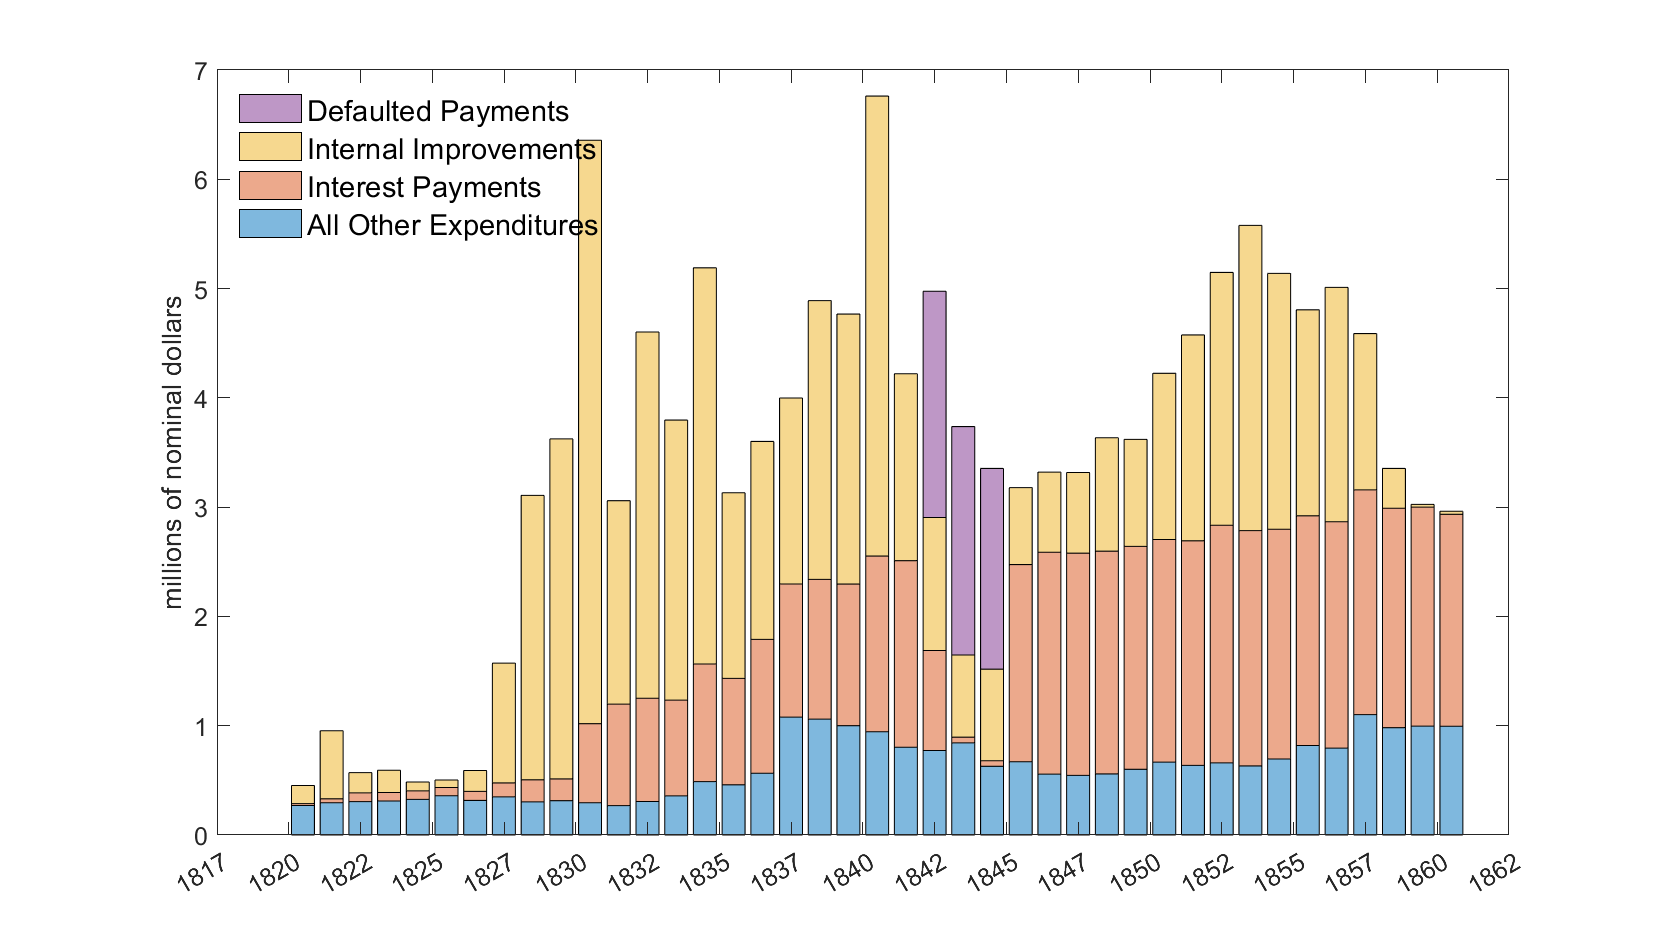
\includegraphics[scale=0.50]{penn_expenditures.png}}
\caption{Pennsylvania Expenditure Decomposed}
\label{fig:penn_expenditures}
\end{figure}

\subsection{Debt and Assets}

\begin{itemize}

\item Between 1825 and 1840, nearly all outstanding debt had been issued to
  fund internal improvements.  Starting in the 1840s, nearly all new debt was
  issued to roll over past debt or cover coupon payments; these refinancing
  loans allowed other revenue to continue financing internal-improvement
  spending.

\item Pennsylvania owned bank stocks, turnpike and bridge stocks, and canal
  and navigation stocks (Figure~\ref{fig:penn_assets}).  In 1843, the State
  sold \$4,169,440 face value of these stocks, receiving only \$1,395,412---
  approximately one-third of face value.

\item Starting in 1835, the State's canals, railroads, and bridges were
  recorded at cost as State Assets, but are not included in
  Figure~\ref{fig:penn_assets}.

\end{itemize}

\begin{figure}[htbp]
\center{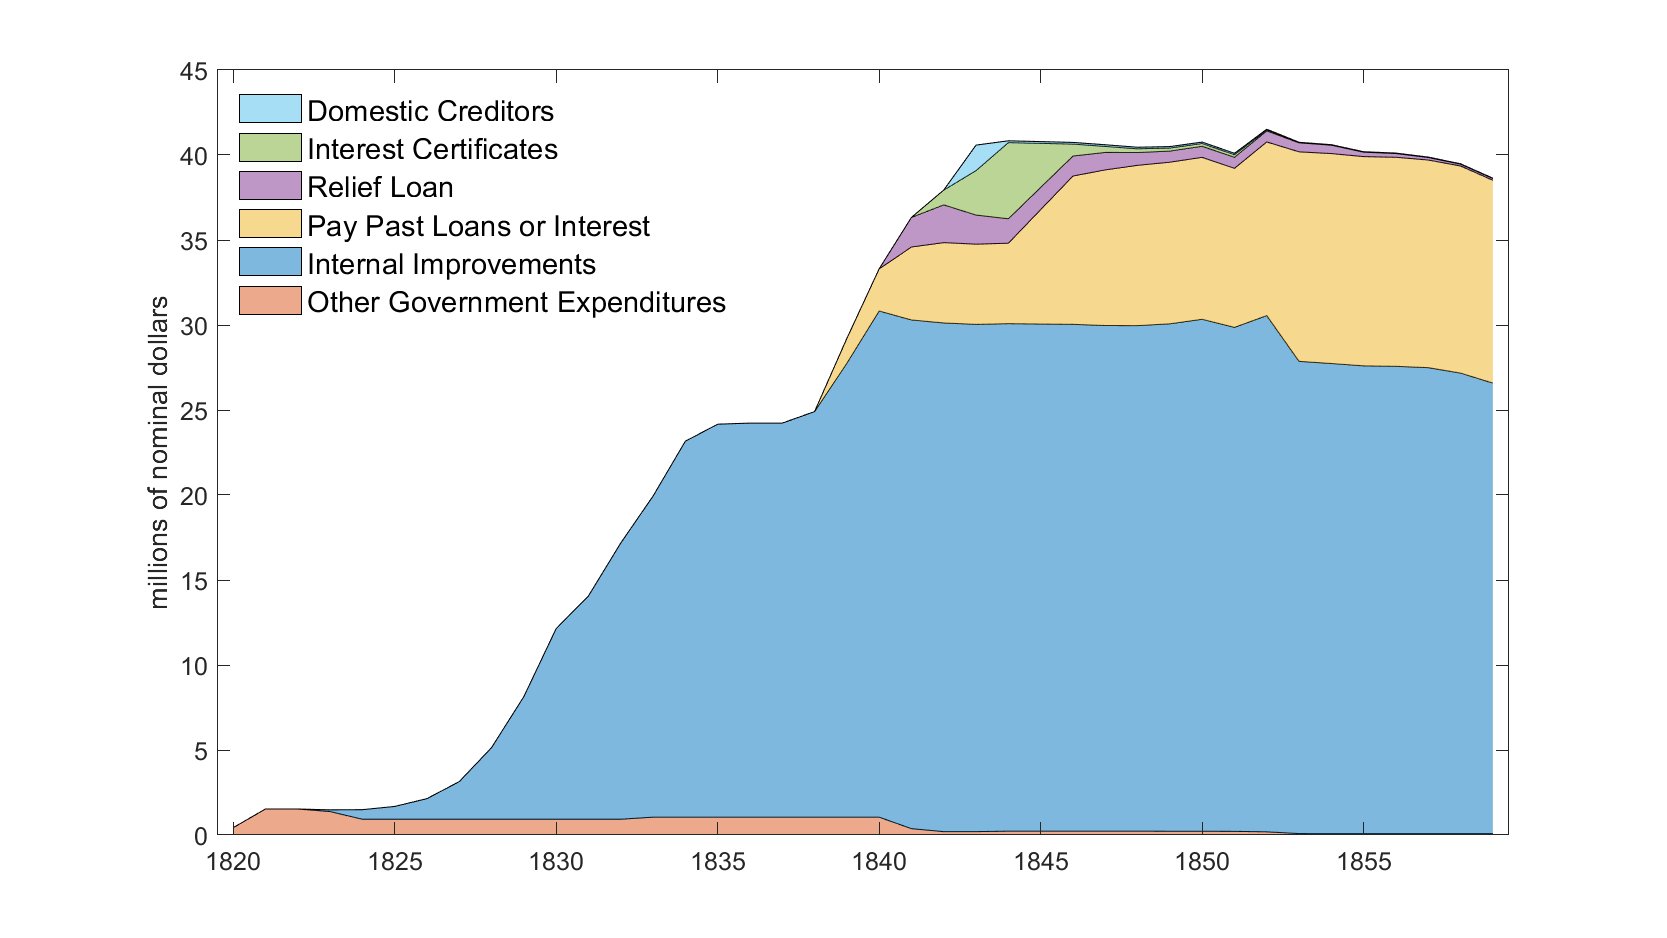
\includegraphics[scale=0.50]{penn_debt_by_purpose.png}}
\caption{Pennsylvania Debt Decomposed by Purpose}
\label{fig:penn_debt}
\end{figure}

\begin{figure}[htbp]
\center{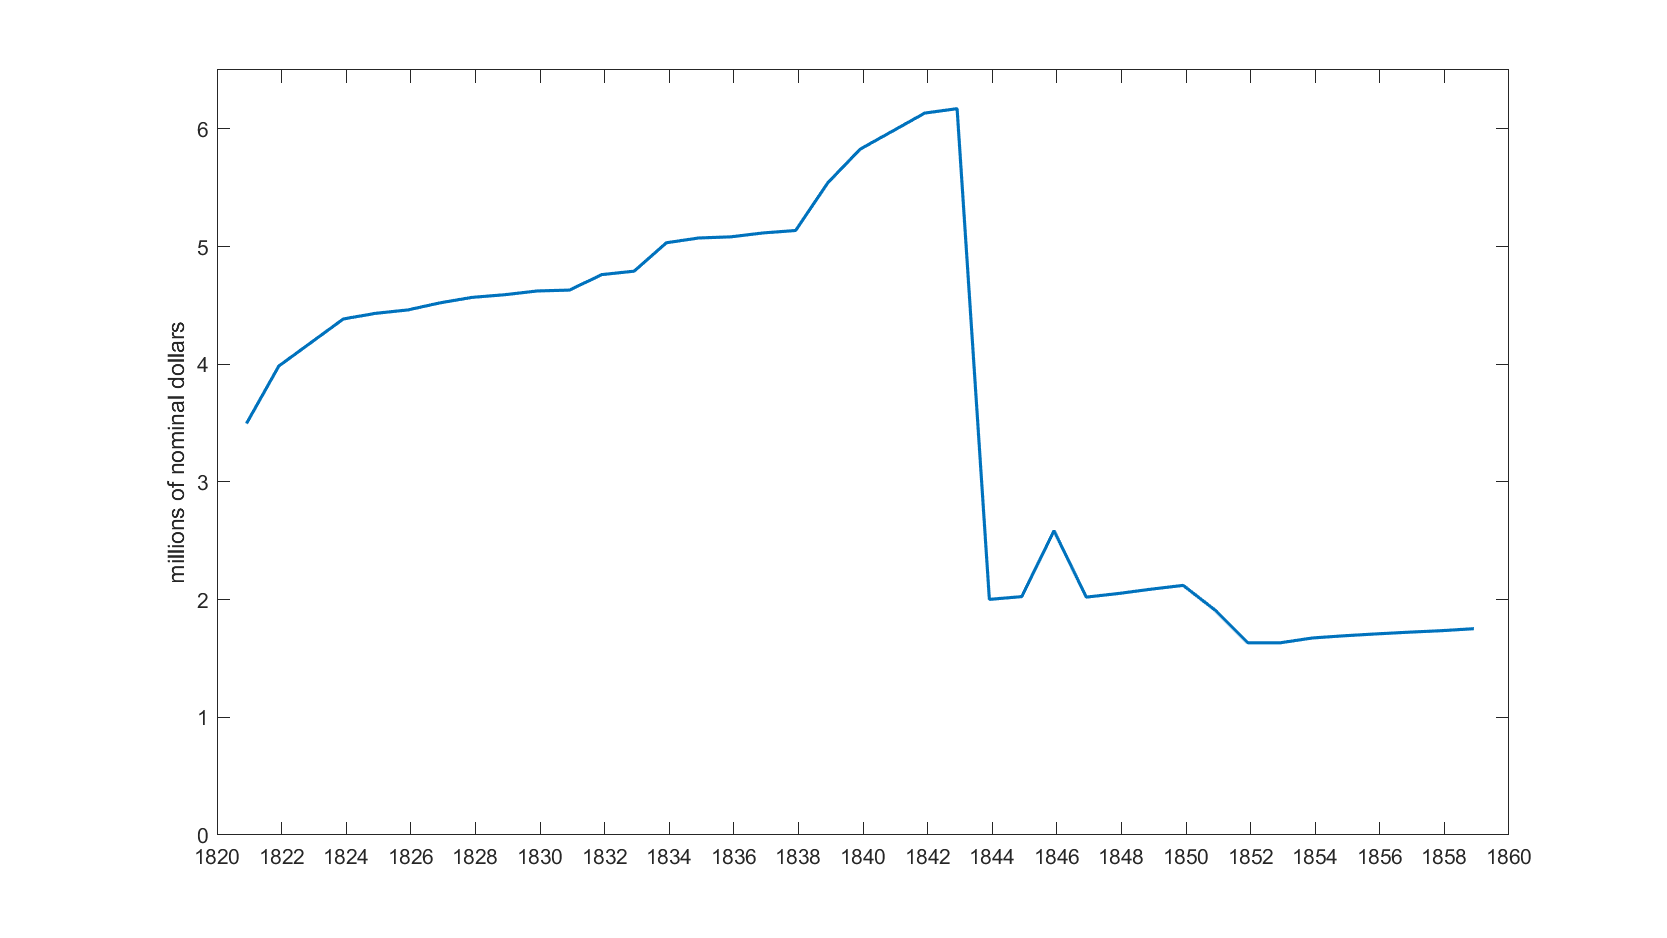
\includegraphics[scale=0.50]{penn_stocks.png}}
\caption{Pennsylvania State Assets, Not Including Public Works}
\label{fig:penn_assets}
\end{figure}

\subsection{The Pennsylvania Canal and Railroad System}

In February~1826, the Pennsylvania Legislature authorized the Main Line of
Public Works---a system of canals and railroads connecting Philadelphia to
Pittsburgh---in direct response to the opening of New York's Erie Canal.
Between 1830 and 1857 the State operated nine canal divisions and two
railroads:

\begin{center}
\begin{tabular}{lrr}
    & Length (miles) & Cost of Construction \\
\cline{2-3}
{\sc Railways} \\
\hspace{3mm} Columbia and Philadelphia        &  82  & \$5,277,278\STRUT\\
\hspace{3mm} Allegheny Portage                &  36  &   2,708,672\\
\cline{2-3}
\hspace{6mm}{\em Railway Total}              & 118  & \$7,985,950\\

{\sc Pennsylvania Canal}\STRUT \\
\hspace{3mm} Eastern Division  &  45  & \$1,737,285\STRUT\\
\hspace{3mm} Juniata Division  & 128  &   3,575,966\\
\hspace{3mm} Western Division  & 103  &   3,173,432\\
\hspace{3mm} Delaware Division &  60  &   1,454,937\\
\hspace{3mm} Susquehanna Division  &  41 &    897,161\\
\hspace{3mm} North Branch Division &  73 &  1,598,379\\
\hspace{3mm} West Branch Division  &  76 &  1,832,583\\
\hspace{3mm} French Creek Division &  49 &    817,780\\
\hspace{3mm} Beaver Division       &  30 &    519,365\\
\cline{2-3}
\hspace{6mm}{\em Canal Total}  & 605  & \$15,606,888\\

Unfinished Improvements  &     & \$8,695,044\STRUT\\
Other Costs              &     &     254,384\\
\cline{2-3}
\hspace{6mm}{\em Grand Total} & & \$32,542,268\\
\end{tabular}
\flushleft{\footnotesize Source: \citet{penn_pub_works_cost_1854}.}
\end{center}

The average construction cost of the Pennsylvania Canal was \$25,797 per mile,
compared with \$19,678 per mile for the Erie Canal.  The comparison highlights
that the Pennsylvania network was both more expensive per mile and---as the
revenue figures show---far less commercially successful.

Table~\ref{table:penn_canal_rev_exp} summarizes the fiscal outcome over the
life of the public works.  The losses were staggering: between 1820 and 1853,
the State spent between \$84 million (our estimate) and \$87 million (the
official estimate) to build, finance, and operate these works, while collecting
only \$25 million in toll revenue.

\begin{figure}[htbp]
\center{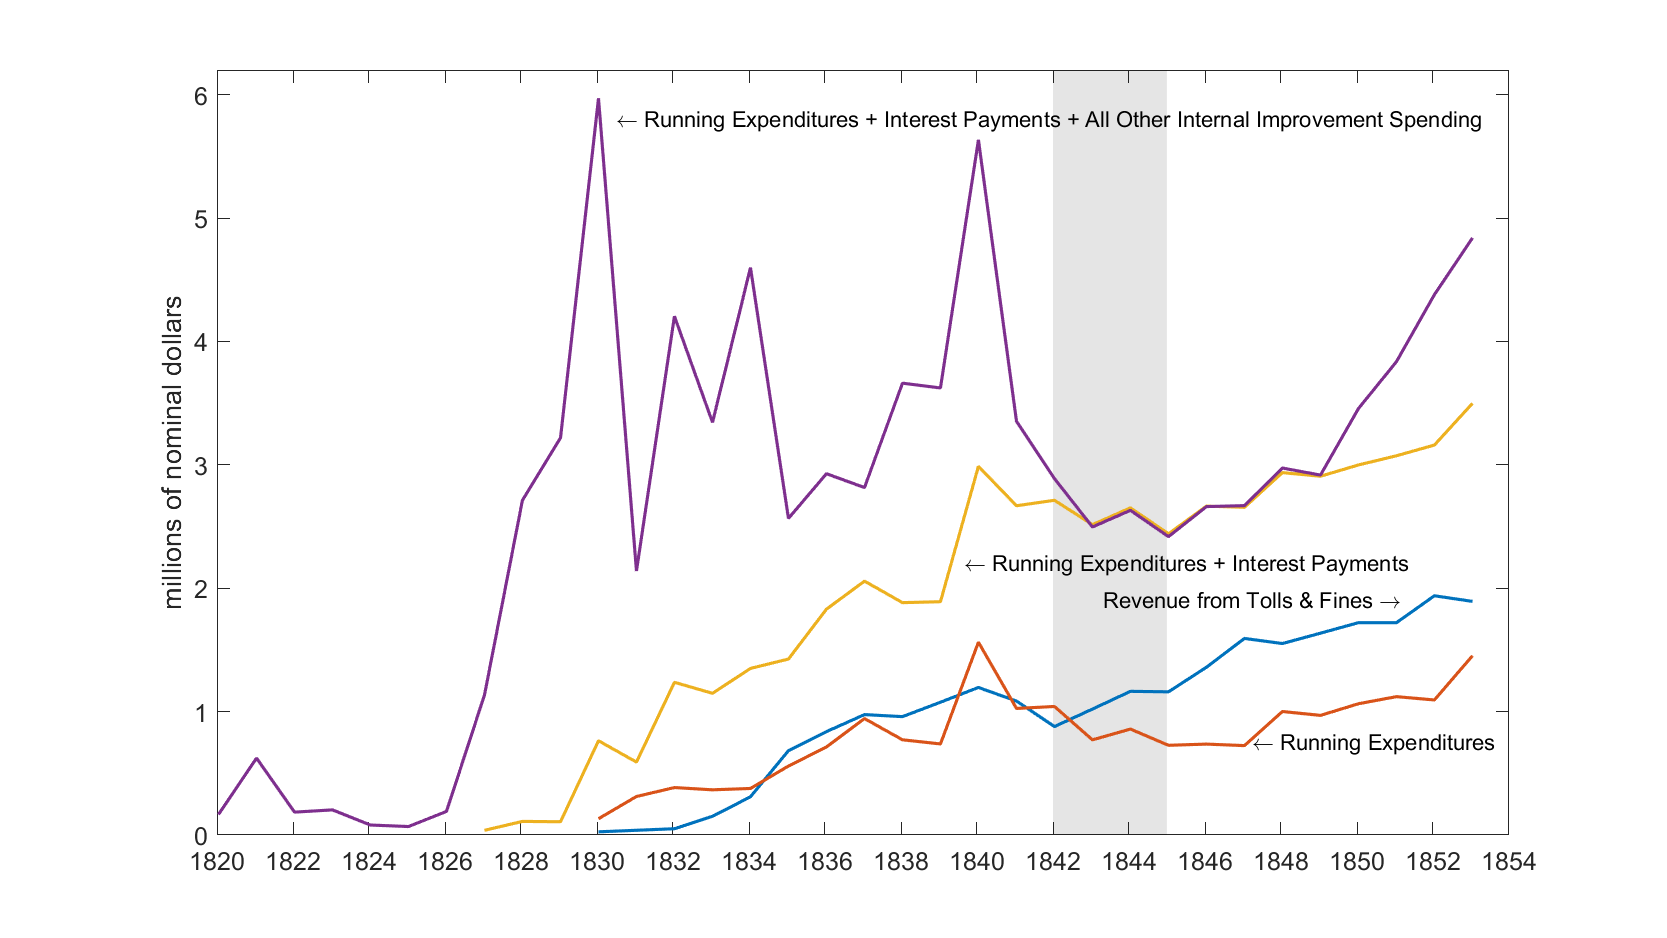
\includegraphics[scale=0.50]{penn_canal_revenue_expend.png}}
\caption{Pennsylvania Canal and Railroad Revenue and Expenditures}
\flushleft{\footnotesize The period of default (1842--1844) is shaded in grey.}
\label{fig:penn_canal_rev_exp}
\end{figure}

\begin{table}[htbp]
\begin{center}
\begin{tabular}{lrr}
                                                    & Official Numbers & Our Numbers\\
\hline
Running Expenses, 1830--1853\STRUT                 & \$19,447,654  & \$19,477,654\\
Interest Payments on Canal \& Railroad Debt, 1827--1853\STRUT
                                                    &  35,157,796   &  35,231,591\\
Construction Costs, 1820--1853\STRUT               &  32,542,268   &  28,954,372\\
\hline
Total Costs\STRUT                                  & \$87,147,717  & \$83,663,617\\
\\
Revenue from Tolls                                  & \$24,995,632  & \$24,995,632
\end{tabular}
\caption{Aggregated Costs and Revenue for the Pennsylvania Canals and Railroads}
\label{table:penn_canal_rev_exp}
\end{center}
\flushleft{\footnotesize Source: \citet{penn_pub_works_cost_1854}.}
\end{table}

After 1842, toll revenues consistently exceeded running expenses, but fell
nowhere near covering interest payments---much less recouping construction
costs.  In 1844 the State offered the works for sale at \$20 million; there
were no takers.  In 1854 another sale attempt likewise failed.  Eventually:
\begin{itemize}
\item On June~25, 1857, the Columbia and Philadelphia Railway, the Allegheny
  Portage Railway, and several canal divisions were sold to the Pennsylvania
  Railroad Company for \$7.5 million.
\item In 1858, the remaining canals and railroads were sold to the Sunbury and
  Erie Railroad Company for \$3.5 million.
\end{itemize}

\subsection{The 1841--1844 Default Crisis}

\subsubsection{Approach to Crisis}

In 1838, 1839, and 1840, Pennsylvania ran budget deficits of \$2.9, \$2.9, and
\$4.8 million, respectively.  In 1841, the deficit was \$2.5 million:
expenditures totaled \$4.2 million (including \$675,000 in loan repayments,
\$1,707,000 in interest, \$1,710,000 in internal improvements, and \$803,000
in ordinary expenditures) against only \$1.7 million in revenue.  The State
was shut out of the bond market.

Figure~\ref{fig:dsp_1840} plots the debt service profile as of December~1840.
Pennsylvania did not face large principal maturities in the 1840s---it was the
promised coupon payments that proved fatal.

\begin{figure}[htbp]
\center{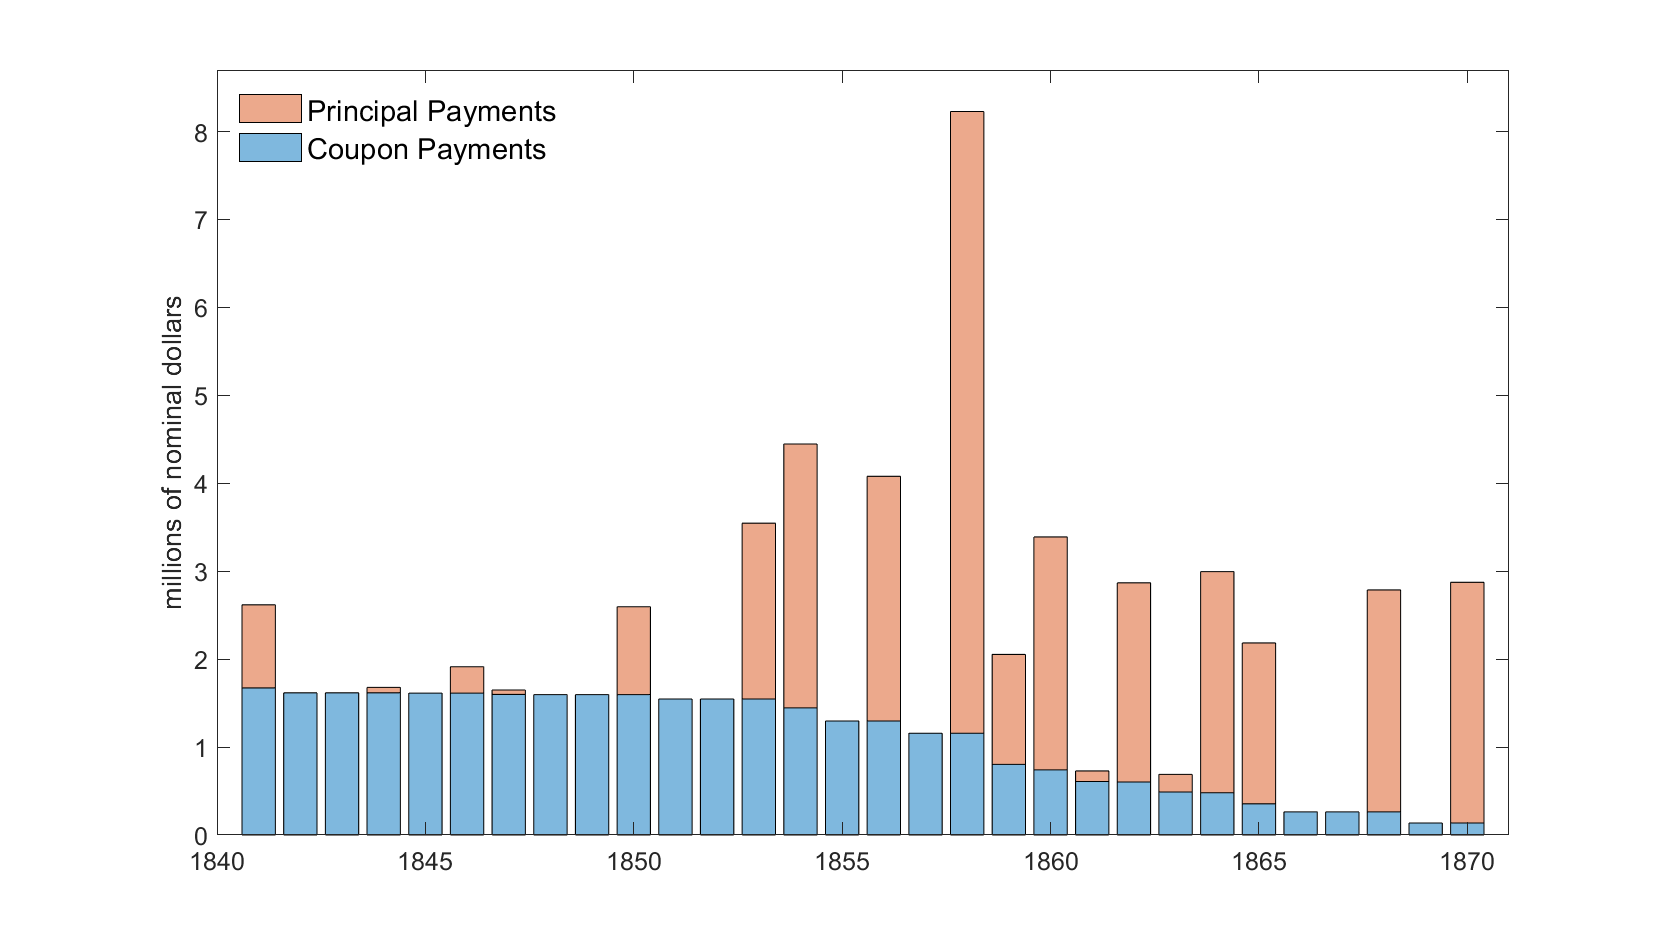
\includegraphics[scale=0.50]{penn_debt_service_profile_1840.png}}
\caption{Debt Service Profile for December~1840}
\label{fig:dsp_1840}
\end{figure}

\subsubsection{1841: Relief Notes}

To meet its 1841 obligations without outright default, Pennsylvania passed the
Relief Note Act of May~4, 1841, authorizing a \$2.22 million``relief loan.''
Banks that subscribed were permitted to issue small-denomination paper currency
(``relief notes'' in \$1, \$2, and \$5 denominations, normally illegal) up to
their subscription amount, and were granted relief from certain state taxes and
penalties for suspending specie payments.  The notes were made receivable for
all debts due to the Commonwealth, effectively making them a state-backed
currency.

\subsubsection{1842--1844: Interest Certificates and Asset Sales}

In February~1842 Pennsylvania met its interest payment, but by August~1 the
treasury was exhausted.  \citet{English_1996} dates the formal default as
August~1842 and the resumption as February~1845.

The State Treasurer issued to bondholders \emph{certificates of stock} equal to
interest then due, bearing 5\% interest and payable on August~1, 1843.
Government contractors and public-works employees unpaid during the crisis were
classified as \emph{domestic creditors}.  County commissioners were instructed
to levy an additional tax of one mill on the dollar on all real and personal
property.

In April~1843, the State sold all of its holdings in bank stocks and other
incorporated companies.  Face value was \$4,169,440; the State received
\$1,395,412---one-third of face value.

\subsubsection{The Discrimination Problem}

The default forced the Commonwealth to choose among:
\begin{enumerate}
\item Failing to pay domestic creditors (contractors, employees),
\item Failing to pay foreign bondholders, or
\item Raising taxes on Pennsylvania citizens.
\end{enumerate}

This was an echo of the discrimination problem Hamilton faced in 1790 when
designing the federal assumption of state debts.  Failing domestic creditors or
raising taxes risked immediate electoral backlash and social unrest; failing
foreign bondholders carried reputational costs that were diffuse and delayed.
In 1842, of the \$34,454,356 in Pennsylvania debt outstanding, approximately
69\% was held by foreigners (overwhelmingly English):

\begin{center}
\begin{tabular}{lr}
Pennsylvania citizens   & \$9,635,613\\
Other U.S.\ citizens   &  1,080,538\\
Foreigners             & 23,738,206\\
\hline
Total                  & \$34,454,357
\end{tabular}
\flushleft{\footnotesize Source: \citet{holders_state_debt_1842}.}
\end{center}

The five largest foreign-creditor countries were England (\$20,026,458),
Holland (\$1,822,266), France (\$570,000), the West Indies (\$563,161), and
Switzerland (\$239,677).  No formal restructuring occurred; the exact mechanism
by which the discrimination problem was resolved remains to be fully
established.

\subsection{Bond Prices}

Figure~\ref{fig:penn_bond_prices} plots Pennsylvania bond prices.  The contrast
with Figure~\ref{fig:nys_bond_prices} for New York is instructive: Pennsylvania
bonds fell further and recovered more slowly, reflecting the deeper fiscal
distress and the actual interruption of payments.

\begin{figure}[htbp]
\center{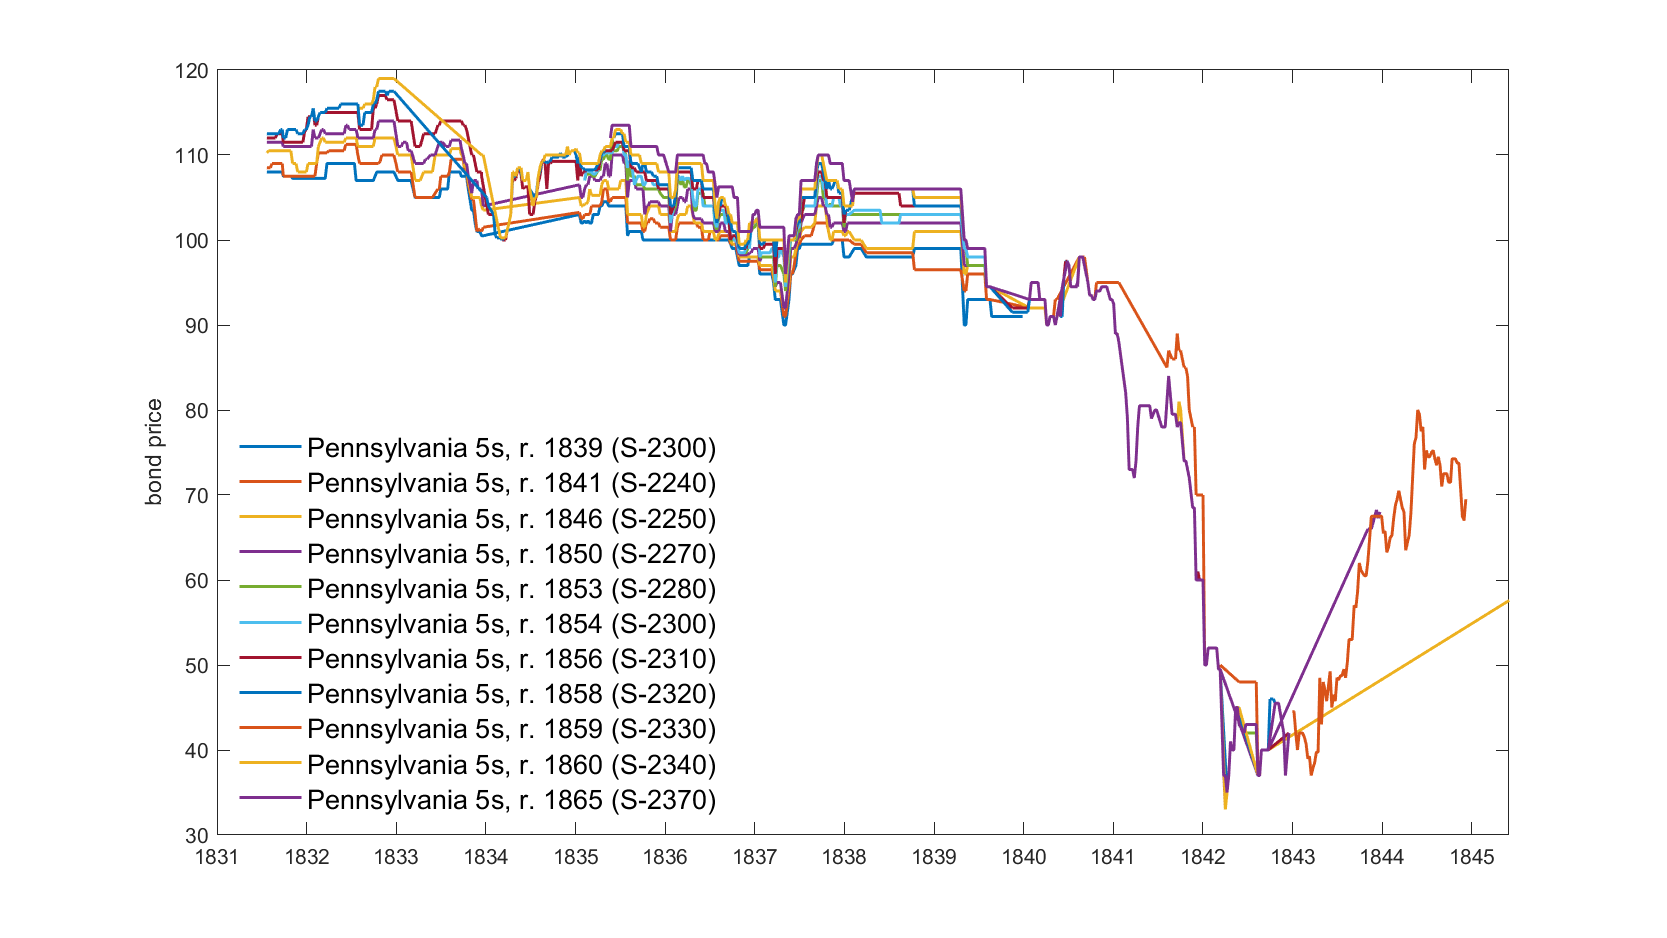
\includegraphics[scale=0.50]{penn_state_debt_prices.png}}
\caption{Prices of Various Pennsylvania State Bonds}
\flushleft{\footnotesize Source: \cite{Sylla_Wilson_Wright}.}
\label{fig:penn_bond_prices}
\end{figure}

\subsection{Unit of Account Issues}

In May~1837, Pennsylvania banks suspended specie payments in response to the
financial panic.  In July~1839, the Legislature resolved that the State would
pay interest in ``lawful money'' (specie), and the Treasury records show
evidence of making up differences between paper and specie values.
Pennsylvania's unit-of-account management stands in contrast to New York's
more consistent adherence to a metallic standard.

%============================================================
\section{The Crisis in Comparative Perspective}
\label{sec:compare}
%============================================================

\subsection{Other Defaulting States}

Beyond Pennsylvania, eight other states and the Florida Territory defaulted
between 1841 and 1843:
\begin{itemize}
  \item \textbf{Maryland}: defaulted with over \$12 million in debt, primarily
    for canal construction.
  \item \textbf{Midwest states} (Indiana, Illinois, Michigan): combined debt of
    approximately \$37 million for railroads and canals.
  \item \textbf{Southern states} (Arkansas, Louisiana, Mississippi): borrowed
    primarily to capitalize state banks.
\end{itemize}
Four states ultimately repudiated all or part of their debts, while three
underwent substantial renegotiations \citep{grinath1997debt}.

\subsection{Patterns of Default}

\citet{wallis2005constitutions} documents that nine of the ten states with the
largest per capita debts defaulted; only New York, Ohio, and Alabama narrowly
avoided this fate.  The pattern is clear: states that had pursued large-scale
infrastructure investment through debt financing, without corresponding tax
increases, were most vulnerable when the post-Panic depression reduced toll
revenues and land values.

\citet{wallis2004sovereign} highlights a critical distinction between states
that defaulted and states with comparable debt levels that avoided default.
Maryland and Pennsylvania both had the \emph{fiscal capacity} to service their
debts through property taxation; the problem was that both were dilatory in
levying adequate taxes.  When crisis forced action, Maryland and Pennsylvania
enacted property taxes and resumed payments with back interest almost
immediately.  By contrast, the northwestern states (Indiana, Illinois,
Michigan) had already implemented high property taxes and genuinely lacked
resources---they were forced to default and partially repudiate.

The New York--Pennsylvania comparison is especially instructive.  Both states
borrowed heavily for canals; both faced fiscal stress in the early 1840s.  The
difference lay partly in project quality (Erie Canal revenues substantially
exceeded Pennsylvania Main Line revenues) and partly in the pre-existing fund
structure that gave New York a balance-sheet cushion that Pennsylvania lacked.

%============================================================
\section{Constitutional Responses}
\label{sec:constitution}
%============================================================

State legislatures throughout the country asked ``how did we get into this
mess?'' and ``how can we prevent this from happening again?''  Although
conditions in every state were unique, the constitutional reforms of the 1840s
shared a common theme: states got into trouble because they pursued taxless
finance, and the solution was to eliminate this option by requiring taxes to be
raised when spending is contemplated \citep{wallis2005constitutions}.

\subsection{New York Constitution of 1846}

New York held a constitutional convention in 1846 that established what scholars
call ``procedural debt restrictions'' in Article~VII:

\begin{enumerate}
  \item A debt limit of \$1 million for ordinary purposes (Section~1).
  \item For debt exceeding this limit (Section~3), the legislature must:
    \begin{itemize}
      \item Contract the debt for a specific, stated purpose;
      \item Enact a tax sufficient to pay the interest and retire the principal
        within 18 years;
      \item Submit the proposed tax to voters for approval in a statewide
        referendum.
    \end{itemize}
  \item Exceptions only for extraordinary emergencies: invasion, insurrection,
    or war.
\end{enumerate}

The Harvard Business School case study \citep{moss2016debt} describes the proposal
by Michael Hoffman as placing ``tight restrictions on state debt, which had
increased sharply over the previous eight years.''  By requiring voter approval
of taxes \emph{before} projects were undertaken, the constitution fundamentally
changed the political calculus of infrastructure investment.

The procedural restrictions did not limit the \emph{amount} of debt a state
could issue; rather, by addressing the timing issue, they created what modern
public finance literature would call a hard budget constraint---making it
impossible for project promoters to promise valuable infrastructure while
deferring the tax burden to the future \citep{grinath1997debt}.

The Constitution of 1846 also mandated the creation of a sinking fund for the
gradual redemption of the General Fund debt; the State retired the last of that
debt in 1878.

\subsection{Pennsylvania Constitutional Amendments of 1857}

Pennsylvania's constitutional response was more delayed.  The state's 1838
constitution did not include comprehensive debt restrictions; major fiscal
reforms came as amendments in 1857, fifteen years after the default.

Article~XI of the amended Pennsylvania Constitution established:

\begin{itemize}
  \item \textbf{Section~1}: Limited state debt to \$750,000 for ``casual
    deficits or failures in revenues.''
  \item \textbf{Section~3}: ``Except the debts above specified \ldots no debt
    whatever shall be created by, or on behalf of the State.''
  \item \textbf{Section~4}: Created a mandatory sinking fund of at least
    \$250,000 annually to retire existing debt.
  \item \textbf{Section~5}: ``The credit of the Commonwealth shall not in any
    manner, or event, be pledged, or loaned, to any individual, company,
    corporation, or association.''
  \item \textbf{Section~6}: Prohibited assuming debts of local governments or
    corporations.
  \item \textbf{Section~7}: Prohibited counties and cities from becoming
    stockholders in corporations or lending their credit.
\end{itemize}

These provisions effectively prohibited Pennsylvania from the practices that
had led to default: borrowing without dedicated revenue sources, investing in
or lending to private corporations, and assuming the debts of other entities.

\subsection{Common Elements Across the Reforms}

The constitutional reforms in New York, Pennsylvania, and other states shared
several features that together eliminated taxless finance:

\subsubsection*{Strict Debt Limits}
Both states imposed absolute limits on state borrowing for ordinary purposes.
New York's \$1 million limit and Pennsylvania's \$750,000 limit were
intentionally restrictive, requiring any significant borrowing to meet
extraordinary criteria or undergo special approval.

\subsubsection*{Prohibition on Lending State Credit}
Both states prohibited the state from pledging its credit to, or becoming a
stockholder in, private corporations---closing the channel through which they
had accumulated contingent and direct debt obligations.

\subsubsection*{Dedicated Revenue Requirements}
Authorized debt had to be accompanied by specific, dedicated tax revenues
sufficient to service and retire it, forcing legislators and voters to confront
the true cost of projects at the time of authorization.

\subsubsection*{Voter Approval}
New York's requirement for a statewide referendum on debt-servicing taxes was
particularly innovative, ensuring that borrowing decisions were made with full
awareness of fiscal consequences.

%============================================================
\section{The ``Taxless Finance'' Problem}
\label{sec:taxless}
%============================================================

\citet{wallis2005constitutions} argues that the fundamental problem was not
the infrastructure investments themselves---many projects, particularly New
York's Erie Canal, were economically sound and generated substantial social
returns.  The problem was the political economy of deferred taxation.

When project promoters could promise infrastructure while claiming it would
``pay for itself'' through tolls or increased land values, voters and
legislators systematically underestimated risks.  Without the requirement to
raise current taxes, several problems emerged:

\begin{enumerate}
  \item \textbf{Optimism bias}: Toll revenue projections were systematically
    optimistic.  Pennsylvania's canal revenues never came close to projections,
    and the state ultimately received only \$11 million in sale proceeds for
    a system that cost \$84--87 million to build, finance, and operate.

  \item \textbf{Risk underestimation}: The probability of adverse economic
    shocks---such as the Panic of 1837---was not adequately factored into
    borrowing decisions.

  \item \textbf{Political agency problems}: Legislators could claim credit for
    visible infrastructure projects while deferring the fiscal costs to future
    administrations.  Both New York and Pennsylvania exhibit this pattern:
    the debts accumulated in the 1820s and 1830s came due in the administration
    of officials who had not made the original borrowing decisions.
\end{enumerate}

The lesson the states drew in the 1840s was that ``taxes must be raised when
spending is contemplated.''  If current taxes are not raised, taxpayers and
politicians may not adequately factor in the risks of higher taxes in the
future \citep{grinath1997debt}.

The contrast between the two states' experiences with unit-of-account management
reinforces this interpretation.  New York's Comptrollers consistently prioritized
maintaining the state's credit standing---paying specie rather than depreciated
paper, even at short-run fiscal cost---while Pennsylvania's management was more
opportunistic.  Fiscal discipline and creditworthiness are complementary.

%============================================================
\section{Long-Run Impact}
\label{sec:longrun}
%============================================================

The constitutional restrictions adopted in the 1840s and 1850s proved
remarkably durable.  No state has experienced a full default since Arkansas in
1933, despite numerous economic downturns over the intervening nine decades.

The reforms established several enduring principles in American state public
finance:

\begin{itemize}
  \item \textbf{Balanced budget requirements}: Most state constitutions now
    require balanced operating budgets.
  \item \textbf{Debt limitations}: States maintain various forms of
    constitutional or statutory debt limits.
  \item \textbf{Voter approval for borrowing}: Many states require voter
    approval for general obligation bonds.
  \item \textbf{Separation of state and private enterprise}: States generally
    cannot invest in or lend to private companies.
\end{itemize}

These restrictions have been criticized at times for limiting states' flexibility
in responding to economic conditions or funding infrastructure.  They represent 
a deliberate choice, made in the wake of fiscal crisis, to constrain the ability
of political actors to defer fiscal burdens to the future.

%============================================================
\section{Conclusion}
\label{sec:conclusion}
%============================================================

The state debt crisis of the 1840s and the constitutional responses it provoked
represent a critical episode in the development of American fiscal federalism.
New York and Pennsylvania---the ``good'' and ``bad'' case studies---illustrate
how similar fiscal strategies (canal-financed through debt, without commensurate
taxation) led to different outcomes depending on project quality, balance-sheet
cushions, and willingness to tax.

Pennsylvania's default was not inevitable: the Commonwealth had the fiscal
capacity to service its debt through property taxation.  The problem, as
\citet{wallis2004sovereign} emphasizes, was the political economy of deferred
taxation---the unwillingness to impose current taxes in the face of projected
(but ultimately unrealized) toll revenues.

The constitutional reforms adopted by New York, Pennsylvania, and other states
addressed this problem by eliminating taxless finance: requiring that taxes be
approved at the time debt is incurred, and prohibiting state investment in or
guarantees of private enterprise.  These institutions have proven remarkably
stable and effective, shaping state fiscal policy nearly two centuries later.

%============================================================
\section{Data Sources}
\label{sec:data}
%============================================================

\subsection*{New York}
\begin{itemize}
  \item Revenue and expenditure data for the General Account: Appendices~I
    and~II of \citet{Sowers_1914} and the \emph{Annual Report of the
    Comptroller} for the State of New York.
  \item Debt outstanding, fund balances, and Treasury balances: \emph{Annual
    Report of the Comptroller}.
  \item Canal Account revenues, expenditures, debt outstanding, and fund
    balances: Table~82, p.~88 of the 1860 \emph{Annual Report of the
    Commissioners of the Canal Fund to the Legislature of the State of New
    York}.
  \item Bond prices: \citet{Sylla_Wilson_Wright}.
  \item Bank Safety Fund details: \citet{Chaddock_1910} and
    \citet{Bodenhorn_1996}; general fund history: \citet{Roberts_1897}.
\end{itemize}

\subsection*{Pennsylvania}
\begin{itemize}
  \item Revenue, expenditure, state balance, and debt data: various issues of
    the \emph{Report on the Finances of the Commonwealth of Pennsylvania Made
    to the Legislature by the Auditor General} and the \emph{Report of the
    State Treasurer upon the Finances of Pennsylvania}.
  \item Canal and railroad cost and revenue estimates: \citet{penn_pub_works_cost_1854}.
  \item Debt ownership: \citet{holders_state_debt_1842}.
  \item Bond prices: \citet{Sylla_Wilson_Wright}.
  \item Default chronology: \citet{English_1996}.
\end{itemize}

In both cases our fiscal records are consistent with the budget constraints
presented in Section~\ref{sec:framework}.

\clearpage
\bibliography{war_finance,../state_defaults}

\end{document}
